\subsection{The \ON{} model in the large-\texorpdfstring{$N$}{N} limit}\label{subsec:0dLargeN}
\begin{disclaimer}
	This subsection is based on \ccite{Steil:2021cbu}.
	The plots of \ccite{Steil:2021cbu} and the underlying numerical data were produced by myself and numerically cross-checked by A. Koenigstein.
	
	The plots, numerical results, and accompanying symbolic computations are included in the digital auxiliary file~\cite{Steil:2023zeroDlargeN}.
	The single thread wall time on an \intel{} for the numeric results of \ccite{Steil:2021cbu} is around three days.
	
	The introduction of this subsection follows Sec. I of \ccite{Steil:2021cbu}.
\end{disclaimer}

After focusing on the limiting case of $O(N=1)$ models in the previous \cref{subsec:0dO1Entropy}, we now want to focus on the other extreme: large and even infinite $N$. 
In this subsection we set out to study zero-dimensional $O(N)$ models at large and infinite $N$ with three computational approaches: direct computation of the underlying integrals \eqref{eq:ON_expectation_value}, $\tfrac{1}{N}$-expansion, and the \frg{} in our newly developed \cfd{} perspective.\bigskip

The $\frac{1}{N}$-expansion is an established ``non-perturbative'' approach to compute observables in \qft{}.
Depending on the context, author, and explicit implementation it is also referred to as large-$N$ expansion, the 't~Hooft limit, or just mean-field approximation.
This method relies on a systematic expansion of characteristic quantities of the theory, like expectation values, correlation functions, and observables, in powers of $\frac{1}{N}$. 
Here, $N$ is the number of different kinds of interacting degrees of freedom of the theory (particle or field types, spins, molecules, color charges \etc{}), which is considered to be large in this context ($1 \lll N$). 
Hence, extensive quantities need to be rescaled by appropriate powers of $N$ in advance to allow for a meaningful $\frac{1}{N}$-expansion.
Although involving an expansion in a small, dimensionless parameter, namely $\frac{1}{N}$, the method is considered to be non-perturbative, because it is also applicable to systems with strong interactions, where an expansion in couplings is doomed to fail.
In consequence, various great successes and precise predictions trace back to this method, see, \eg{},\ \ccite{tHooft:1973alw,Veneziano:1979ec,Witten:1979vv,Witten:1979kh,Gross:1974jv,Maldacena:1997re,DAttanasio:1997yph,Keitel:2011pn,Grossi:2019urj} or the review~\cite{Moshe:2003xn} \dash{} in some cases maintaining predictive power even for systems, where $N$ is surprisingly small.
However, the large-$N$ expansion and especially retaining only its zeroth-order contribution \dash{} the infinite-$N$ limit \dash{} also comes with some limitations and certain fundamental characteristics of a (quantum) field theoretical or statistical models, like the convexity of the $\tfrac{1}{N}$-rescaled effective action may be altered.

In order to elucidate some of these aspects and interesting consequences, we study the large-$N$ expansion and the infinite-$N$ limit within two totally different setups.
On the one hand, we perform a conventional saddle-point expansion of the functional integral (partition function) by assuming that $N$ is large (or even infinite)~\cite{Arfken:2005,Keitel:2011pn}.
On the other hand, we study the same problem within the \frg{} approach, also considering large and/or (in)finite $N$, see, \eg{}, \ccite{Tetradis:1995br,Litim:1995ex,DAttanasio:1997yph,Litim:2002cf,Fejos:2012rz,Litim:2016hlb,Yabunaka:2017uox,Yabunaka:2018mju,Yabunaka:2021fow,Grossi:2019urj,Grossi:2021ksl} for material regarding the infinite-$N$ limit in the \frg{} framework.

To keep our discussion as simple as possible we limit our discussion to the sober and exactly solvable zero-dimensional $O(N)$ model \dash{} the gift that keeps on giving.
A lot of aspects of the large-/infinite-$N$ limit have been discussed already within this setup, \cf{} \ccite{Hikami:1978ya,Bessis:1980ss,DiVecchia:1990ce,Nishigaki:1990sk,Schelstraete:1994sc,Zinn-Justin:1998hwu,Keitel:2011pn} \dash{} especially for quartic actions (potentials).

Within this work we use the zero-dimensional $O(N)$~model at large $N$ to highlight the following aspects:
	\begin{enumerate}
		\item	Considering a rather simple \dash{} but non-analytic \dash{} one-parameter family of classical actions (potentials) as a new purpose-build test case, we demonstrate that there is a narrow line between a straightforward applicability of the large-$N$ saddle-point expansion and a total failure of this method. 
		In our zero-dimensional pedagogical and tailor made example, this point of failure is easy to detect. 
		However, it may serve as a warning for applications of the large-$N$ limit and the corresponding saddle-point expansion of the functional integral in higher-dimensional scenarios, where it is not necessarily easy to judge, if all requirements for a meaningful $\tfrac{1}{N}$-expansion are fulfilled.
		Note that in our large-$N$ applications of \cref{chap:GN,chap:QMM} we use this limit \dash{} the mean-field \dash{} approximation as a technical simplification to study fermionic fluctuations.
		We do not assess or discuss whether or when such a limit is justified when describing physical systems, since we are not interested in describing physical systems in this limit.
		
		\item	Switching perspectives to the \frg{}  formalism, we make use of the fact that the corresponding \frg{} flow equation is exact for the zero-dimensional $O(N)$~model. 
		Being ``exact'' in this context means, that truncating the flow equation is not necessary (for finite and infinite $N$), since the involved \pdes{}, can be solved numerically, with our at this point firmly established methods of \cref{subsec:FRG-formulationONmodel,subsec:0dONresults}.
		Within our fluid-dynamic framework, we show that the \frg{} flow in the infinite-$N$ limit is purely advection driven, while diffusive contributions enter only at finite $N$.
		This also generalizes to higher space-time dimensions.
		
		As a direct consequence, depending on the classical action (potential) \dash{} \uv{} \ic{}, the infinite-$N$ \frg{} flows tend to form or sustain non-analyticities of different kinds, \eg{}, shock and rarefaction waves or jump discontinuities, \cf{} \cref{subsec:hydroAdvection,subsec:hydroEuler} and \ccite{Grossi:2019urj,Grossi:2021ksl}. 
			
		We find that for our toy model with non-analytic classical action, shock and rarefaction waves are present and the problem encountered at the \uv{} initial scale involves two Riemann problems.
		But we do not stop by turning the calculation of ordinary $N$-dimensional integrals with spherical symmetry for expectation values into a fluid-dynamical problem. 
		We also demonstrate that the (non\nobreakdash-)applicability of the large-$N$ saddle-point expansion translates into the (collision) freezing of interacting shock waves in these fluid-dynamic \frg{} flows.
					
		\item	Still working in the \frg{} fluid-dynamic framework, we also demonstrate that the inclusion of the radial \sigmaMode{}, thus switching from infinite-$N$ to arbitrary but finite $N$, totally changes the physics of the system. 
		In the infinite-$N$ limit, we explicitly show by numerical calculations that convexity and smoothness are not necessarily realized for $\tfrac{1}{N}$-rescaled \ir{} potentials, which effectively violates the \cmwhTheoremWithRefs, \ie{}, a special zero-dimensional version of the theorem~\cite{Moroz:2011thesis,Koenigstein:2021syz}.
		Interestingly, as soon as $N$ is finite, the highly non-linear diffusive contribution of the radial \sigmaMode{} unavoidably restores convexity and smoothness of the $\tfrac{1}{N}$-rescaled \ir{} potentials.
		Hence, the large-$N$ expansion with finite $N$ and the infinite-$N$ limit (only retaining the zeroth-order of the $\tfrac{1}{N}$-expansion) may lead to two fundamentally different results.
		We will encounter a qualitatively similar situation in \cref{subsubsec:variableN} for the \gnym{}.
		
		\item	As a last aspect, we also highlight further direct consequences of our fluid-dynamic interpretation of \frg{}  flows. 
		Utilizing the method of characteristics~\cite{polyanin2016handbook,LeVeque:2002,Delgado2006Aug} and the Rankine-Hugoniot condition~\cite{Rankine:1870,Hugoniot:1887}, see also \cref{subsec:MoC}, we directly track the locations of shock and rarefaction waves in the field space derivative of the scale-dependent potential during the \rg{}  flows.
		Applications of the aforementioned methods in \grg{}  studies can be found in, \eg{}, \ccite{Tetradis:1995br,Litim:1995ex,Aoki:2014,Aoki:2017rjl,Grossi:2019urj}.
		
		Interacting shock and rarefaction waves, but also diffusive processes \dash{} as discussed at length in the previous \cref{subsec:0dO1Entropy} \dash{} go hand in hand with the rise of entropy in fluid-dynamic problems, \cf{} \cref{subsec:hydroAdvection}.
		Using the \cfd{} framework and the \tvni{} property, we are able to provide an entropy function in the $N\rightarrow\infty$ limit.
	\end{enumerate}

At this point, we remark that our research in this subsection was partially influenced by the excellent publication~\cite{Grossi:2019urj} on the infinite-$N$ limit of the \frg{}  flow equations of the $O(N)$~model in three Euclidean space-time dimensions and the interpretation of these \frg{} flows as advection equations, which can develop different kinds of discontinuities~\cite{Grossi:2019urj}. 
The application of the method of characteristics in the large-$N$ limit of \frg{}  flow equation predates the explicit identification and detailed understanding of infinite-$N$ \frg{} flow equations as advection equations and goes back (to the best of our knowledge) to \ccite{Tetradis:1995br,Litim:1995ex}.
The authors of \ccite{Grossi:2019urj}, E.~Grossi and N.~Wink, were involved in the first two parts of our series of publications~\cite{Koenigstein:2021syz,Koenigstein:2021rxj} and also worked together with F.~Ihssen and J.~M.~Pawlowski on calculations in the \qmm{} in the infinite-$N$ limit~\cite{Grossi:2021ksl,Ihssen2020,Ihssen:2023xlp}, which was also based on a fluid dynamic interpretation of \frg{} flows.

In addition, we thank the referee of \ccite{Steil:2021cbu} for pointing out that there are recent works, which also deal with the shortcomings of the standard infinite-$N$ limit in the context of F\rg{} and link this to non-analytic structures in the fixed-point potential~\cite{Yabunaka:2018mju,Yabunaka:2021fow}.
An interesting future prospect is certainly to draw a connection between our works in the fluid-dynamic framework and these results.\bigskip

The remainder of this subsection is structured as follows.
In \cref{subsubsec:0dLargeNON} we discuss the zero-dimensional $O(N)$ model at large $N$ and in the paragraph \customref{paragraph:RP}{An instructive toy model} we introduce the test case/action we will consider thereafter.
In \cref{subsubsec:saddle_point} we discuss the $\frac{1}{N}$-saddle-point-expansion for this test case and in \cref{subsubsec:FRGlargeN} we discuss the corresponding \frg{} flows.

\clearpage
\subsubsection{The zero-dimensional \texorpdfstring{$O(N)$}{O(N)} model at large N}\label{subsubsec:0dLargeNON}
\begin{disclaimer}
	This subsubsection follows Sec. II of \ccite{Steil:2021cbu}.
\end{disclaimer}
\vspace{-3em}%
\paragraph{Free theory}\phantomsection\label{paragraph:free_theory}\mbox{}\\%
For later reference, we recapitulate some results for the massive non-interacting free theory.
The action of the corresponding $O(N)$~model is given by
\begin{align}
	U_\mathrm{free} ( \rho ) \equiv m^2 \rho \, ,
\end{align}
with the positive non-zero ``mass'' $m$. 
The expectation values \eqref{eq:ON_expectation_value} can be computed analytically in terms of Gamma functions resulting in
\begin{align}
	\big\langle ( \vec{\phi}^{\, 2} )^0 \big\rangle = \, & \big\langle 1 \big\rangle = 1 \, ,	\\[.25em]
	\big\langle ( \vec{\phi}^{\, 2} )^n \big\rangle = \, & \frac{N + 2 n - 2}{m^2} \, \big\langle ( \vec{\phi}^{\, 2} )^{n-1} \big\rangle \, ,\qquad\text{for}\quad n > 1\, .
\end{align}
For the \ipi{} correlation functions this result implies
\begin{align}
	\Gamma^{(2)} = m^2 \, ,	\qquad\text{and}\qquad	\forall n \neq 2 \quad \Gamma^{(n)} = 0 \, ,	\label{eq:free_Gamma}
\end{align}
where we used the short-hand notation $\Gamma^{(n)} \equiv \, \Gamma^{(n)}_{\varphi_i \ldots \varphi_i}$ from \cref{sec:0dON}.
In their interpretation as interaction vertices these results for $\Gamma^{(n)}$ are rather intuitive for a ``massive non-interacting'' theory, which has only a non-vanishing \ipi{} two-point function, because the underlying probability distribution is Gaussian.

\paragraph{Reformulation for large-\texorpdfstring{$N$}{N}}\phantomsection\label{paragraph:zerodOinfRescaling}\mbox{}\\%
For computations at large $N$ and in the limit ${N \rightarrow \infty}$ the rescaling
\begin{align}
	&	\rho \mapsto y = \tfrac{1}{N} \, \rho \, ,	&&	U ( \rho ) \mapsto V ( y ) = \tfrac{1}{N} \, U ( \rho ) \, ,	\label{eq:rescalings}
\end{align}
has proven particularly useful, see, \eg{}, \ccite{Keitel:2011pn,Grossi:2019urj}, because both $y$ and $V ( y )$ are of $\order ( N^0 )$. The expression \eqref{eq:ON_expectation_value} for $\langle( \vec{\phi}^{\, 2} )^n\rangle$ reads
\begin{align}
	\langle ( \vec{\phi}^{\, 2} )^n \rangle = \, & \frac{2^n N^n \int_0^\infty \dif y \, y^\frac{(N - 2)}{2} \,  y^n \, \eu^{-N V ( y )}}{\int_0^\infty \dif y \, y^\frac{(N - 2)}{2} \, \eu^{-N V ( \rho )}} =\,\frac{2^n N^n \int_0^\infty \dif y \, y^{n - 1} \, \eu^{- N \, [ V ( y ) - \frac{1}{2} \ln ( y ) ]}}{\int_0^\infty \mathrm{d} y \, y^{-1} \, \eu^{- N \, [ V ( y ) - \frac{1}{2} \ln ( y ) ]}} \, ,	\label{eq:ON_expectation_value_largeN}
\end{align}
in terms of $y$ and $V ( y )$ and we note $\langle ( \vec{\phi}^{\, 2} )^n \rangle=\order ( N^n )$. For certain potentials $V(y)$ the involved integrals
	\begin{align}
		I_n^N [ V ] \equiv \int_0^\infty \dif y \, y^{n - 1} \, \eu^{- N \, [ V ( y ) - \frac{1}{2} \ln ( y ) ]}	\label{eq:In_largeN}
	\end{align}
can be solved in terms of known functions, see, \eg{}, \ccite{Keitel:2011pn,Koenigstein:2021syz,Keitel:2011pn} as well as \cref{paragraph:RP}, and/or they can be computed in the limit ${N \rightarrow \infty}$ by means of a saddle-point expansion, see \cref{subsubsec:saddle_point} and \cref{app:saddle_point_app}.
\clearpage

\fullWidthTwoColumnSubFigures%
	[!t] % Placement
	{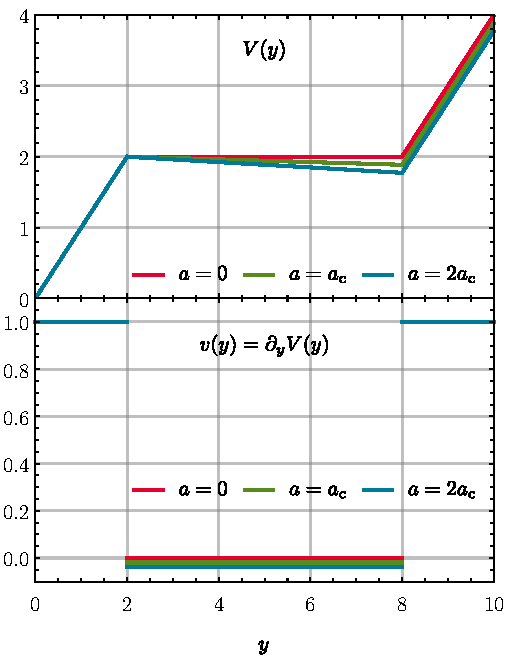
\includegraphics[width=\subcaptionFigureWidth+0.145cm]{0d/figures/Vofy.pdf}} % left figure
	{\vspace{-0.06cm}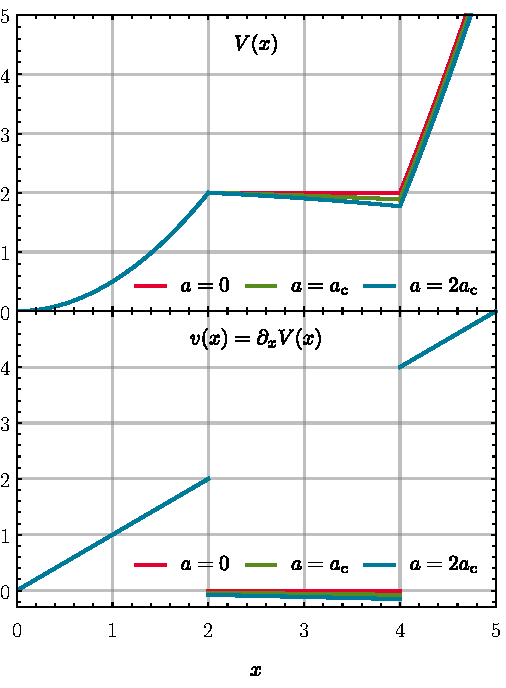
\includegraphics[width=\subcaptionFigureWidth-0.145cm]{0d/figures/Vofx.pdf}} % Right figure
	[fig:Vofy,fig:dVofy,fig:Vofx,fig:dVofx]
	{%
		The potential $V ( y )$ from \cref{eq:RP_Vofy} in the upper, left panel \subref{fig:Vofy} and its $y$-derivative $v ( y ) = \partial_y V ( y )$ from \cref{eq:RP_vofy} in the lower, left panel
		\subref{fig:dVofy} as well as the corresponding potential $V ( x )$ from \cref{eq:RP_Vofx} in the upper, right panel \subref{fig:Vofx} and its $x$-derivative $v ( x ) = \partial_x V ( x )$ from \cref{eq:RP_vofx} in the lower, right panel \subref{fig:dVofx} for selected values of the parameter $a$ \dash{} with ${a_\mathrm{c}\simeq 0.018951}$ from~\cref{eq:a_critical}.
		\fromFigs{1 and 3}{zerod3}
	}%
	{fig:Vofxy}
\FloatBarrier

\paragraph{An instructive toy model}\phantomsection\label{paragraph:RP}\mbox{}\\%
In this paragraph we present an explicit $O(N)$~model, respectively its $\frac{1}{N}$-rescaled self-interaction potential $V(y)$, which turns out to be a rather instructive toy model when studied at large and infinite $N$. We consider a family of piecewise linear potentials
	\begin{align}
		V ( y ) =
		\begin{cases}
			y							&	\text{for} \quad 0 \leq y \leq 2 \, ,\\
			- a \, y + 2 \, ( a + 1 )	&	\text{for} \quad 2 < y \leq 8 \, ,\\
			y - 6 \, ( a + 1 )			&	\text{for} \quad y>8 \, ,
		\end{cases}	\label{eq:RP_Vofy}
	\end{align}
with a parameter $a\geq0$. The first derivative of $V ( y )$ presents as a simple piecewise constant function in the $\tfrac{1}{N}$-rescaled invariant $y$
	\begin{align}
	v ( y ) = \partial_y V ( y ) =
	\begin{cases}
		1	&	\text{for} \quad 0 \leq y \leq 2 \, ,\\
		- a	&	\text{for} \quad 2 < y \leq 8 \, ,\\
		1	&	\text{for} \quad y>8 \, ,
	\end{cases}	\label{eq:RP_vofy}
\end{align}
which is very similar to the \ic{} (32) studied in \ccite{Grossi:2019urj}. The potential \eqref{eq:RP_Vofy} and its $y$-derivative \eqref{eq:RP_vofy} are plotted in \cref{fig:Vofy,fig:dVofy} for illustrative purposes.
In \cref{fig:Vofx,fig:dVofx}, we also plot the potential and its derivative as functions of the rescaled field $x$, where $\tfrac{1}{2} \, x^2 \equiv y\equiv \tfrac{1}{2N} \, \vec{\phi}^{\, 2}$, which might be more familiar after the preceding discussions of \cref{sec:0dON}.
We recognize such an initial value problem with piecewise constant \ics{} involving a set of contact discontinuities as a series of Riemann problem in the context of conservation equations and \cfd{}, \cf{} \cref{sec:conservationLaws}.
When considering \cref{eq:RP_vofy} as the \ic{} of a conservation equation in $y$, \cf{} \cref{paragraph:infiniteNflowsY}, we are faced with two Riemann problems (one at $y=2$ and one at $y=8$) at the \uv{} initial scale.

This model has several interesting properties:
\begin{enumerate}
	\item	The expectation values of \cref{eq:ON_expectation_value_largeN} can be evaluated in terms of known functions.
	In the limit ${N \rightarrow \infty}$ the \ipi{} correlation functions can be computed analytically for all $a\geq0$.
	We will discover within this subsection that there are two distinct parameter regimes, which are particularly interesting when studying this problem within the saddle-point and \frg{} frameworks.
	
	\item	For certain parameters $a$, which are smaller than some critical value $a_\mathrm{c}$, the \ipi{} correlation functions $\Gamma^{(n)}$ \dash{} the underlying expectation values \eqref{eq:ON_expectation_value_largeN} \dash{} can be computed by means of a saddle-point expansion.
	For $a \geq a_\mathrm{c}$ the saddle-point expansion is not applicable.
	This is discussed in detail in the following \cref{subsubsec:saddle_point}.
	
	\item	The model under consideration presents initially as two Riemann problems in the \frg{}  (fluid-dynamic) framework.
	The distinct parameter regimes, ${0 \leq a \leq a_\mathrm{c}}$ and $a > a_\mathrm{c}$, present with qualitatively different \frg{} flows.
	The interpretation involving Riemann problems, its numerical solution, and its consequences are discussed in detail in \cref{subsubsec:FRGlargeN}.
	At this point we also want to remind the reader of the methodological introduction of \cref{subsec:hydroAdvection,subsec:hydroEuler} which will be of great relevance for this subsection \dash{} the discussion of \frg{} flows at large and infinite $N$.
\end{enumerate}\bigskip

\fullWidthTwoColumnFigureTable%
	[!t] % Placement
	{0d/figures/fofy.pdf} % Figure
	{fig:sp_fofy} % Figure label
	{%
		Plot of ${f ( y ) = V ( y ) - \tfrac{1}{2} \ln ( y )}$ for the potential~\eqref{eq:RP_Vofy} for selected values of the parameter $a$ \dash{} with ${a_\mathrm{c}\simeq 0.018951}$ from~\cref{eq:a_critical}. The local minima of $f ( y )$ are located at $y_0 = \tfrac{1}{2}$ and $y_{0, 2} = 8$, where $y_0$ ($y_{0, 2}$) presents as the unique global minimum for $0 \leq a < a_\mathrm{c}$ ($a > a_\mathrm{c}$). At $a = a_\mathrm{c}$ both minima coincide and present both as global minima of $f ( y )$. The non-analyticity of $f ( y )$ in $y_{0, 2} = 8$ inherited from the piecewise definition of $V ( y )$ is clearly visible in the plot.
		\fromFig{2}{zerod3}%
	} % Figure caption
	{%
		\renewcommand{\arraystretch}{1.15}
		\small
		\begin{tabular}{l | c c c}
			\toprule
			$N$			&	$a = 0$		&	$a = a_\mathrm{c}$	&	$a = 2\, a_\mathrm{c}$\\
			\midrule
			$2$			&	$0.356907$	&	$0.327332$ 			&	$0.299162$\\
			$32$		&	$0.962306$	&	$0.475285$			&	$0.087158$\\
			$\infty$	&	 $1$		&	$1$					&	$0.0625$\\
			\bottomrule
		\end{tabular}
	} % Table content
	{tab:Gamma2N}% Table label
	{%
		Reference values for selected $N$ and $a$ of ${\Gamma^{(2)} = N ( \langle \vec{\phi}^{\, 2} \rangle )^{- 1}}$ computed with the expressions \eqref{eq:InNV_a0} and \eqref{eq:InNV} as well as their large $N$ asymptotics.
		The exact analytical results are in some cases rather lengthy and therefore we present in those cases only six decimal digits for readability.
		\fromTab{I}{zerod3}%
	} % Table caption
For now, we turn to the computation of the correlation functions of the model under consideration.
Solutions in terms of known functions for the necessary integrals \eqref{eq:In_largeN} for the potential \eqref{eq:RP_Vofy} are presented in \cref{app:RP_integrals}.
In the limit ${N \rightarrow \infty}$ the direct computations of \cref{app:RP_integrals} revealed two distinct regimes in parameter space separated by
\begin{align}
	a_\mathrm{c} = \tfrac{1}{4} - \tfrac{1}{3} \ln ( 2 ) \simeq 0.018951 \, .	\label{eq:a_critical}
\end{align}
For the infinite-$N$ limit of the expectation values \eqref{eq:ON_expectation_value} we find,
\begin{align}
	\lim_{N \rightarrow \infty} \tfrac{1}{N^n} \, \big\langle ( \vec{\phi}^{\, 2} )^n \big\rangle =
	\begin{cases}
		1 \, ,		&	\text{for} \quad 0 \leq a \leq a_\mathrm{c} \, ,\\
		16^n \, ,	&	\text{for} \quad a>a_\mathrm{c} \, ,
	\end{cases}
\end{align}
For the corresponding \ipi{} correlation functions this implies in the limit ${N \rightarrow \infty}$
\begin{align}
	\Gamma^{(2)} =	\label{eq:two-point_exact}
	\begin{cases}
	1 \, ,				&	\text{for} \quad 0 \leq a \leq a_\mathrm{c} \, ,
	\\
	\tfrac{1}{16} \, ,	&	\text{for} \quad a>a_\mathrm{c} \, ,
\end{cases}
\end{align}
as well as for all $a \geq 0$ 
\begin{align}
	\forall n \neq 2 \quad \Gamma^{(n)} = 0 \, .	\label{eq:n-point_exact}
\end{align}
Thus, in the limit ${N \rightarrow \infty}$ and in terms of \ipi{} vertices the current model under consideration presents as a massive non-interacting theory for all $a \geq 0$, \cf{} \cref{eq:free_Gamma}.
The situation for $0\leq a<a_\mathrm{c}$ and the corresponding ``mass'' as well as the origin of the critical value $a_\mathrm{c}$ can be understood intuitively in the context of the saddle-point expansion discussed in \cref{subsubsec:saddle_point}.
The situations for $a =a_\mathrm{c}$ and $a >a_\mathrm{c}$ are more involved and not accessible with a saddle-point expansion. 
However, a study in the \frg{}  framework is possible and rather instructive as we will demonstrate in \cref{subsubsec:FRGlargeN}.
In terms of correlation functions the theory undergoes a first-order phase transition at $a_\mathrm{c}$ when varying the external parameter $a$, \cf{} Sec.~III.C of \ccite{Grossi:2019urj} and references therein.

For finite $N$ higher-order \nptFunctions{} do not vanish and the theory is of ``interactive type'', but in the scope of this subsection we nevertheless mainly focus on $\Gamma^{(2)}$ \dash{} especially when it comes to numerical computations. In \cref{tab:Gamma2N} we summarize several (exact) reference values for $\Gamma^{(2)}$ for later use.

\FloatBarrier
\subsubsection{The saddle-point expansion at large \texorpdfstring{$N$}{N}}\label{subsubsec:saddle_point}
\begin{disclaimer}
	This subsubsection follows Sec. III of \ccite{Steil:2021cbu}.
\end{disclaimer}
In this subsubsection we will analyze the instructive toy model of \cref{paragraph:RP} within a saddle-point approximation for large $N$.
In \cref{app:saddle_point_app} we discuss the large-$N$ saddle-point expansion of integrals like \eqref{eq:In_largeN} concluding in the asymptotic series \eqref{eq:SPapp_series} for $\langle ( \vec{\phi}^{\, 2} )^n \rangle$.
To apply the series \eqref{eq:SPapp_series} to the interaction potential \eqref{eq:RP_Vofy} of the model under consideration, we first have to compute the global minimum $y_0$ of the exponents of the integrands in \cref{eq:ON_expectation_value_largeN},
\begin{align}
	f ( y ) = V ( y ) - \tfrac{1}{2} \ln ( y ) \, ,\label{eq:fofy}
\end{align}
and check for analyticity of $f ( y )$ and $g ( y ) = y^{n - 1}$ around $y_0$.
The function $f ( y )$ for the model under consideration is plotted in \cref{fig:sp_fofy} for different parameters $a$.

There is always a minimum on the first section (${0 \leq y \leq 2}$) of the piecewise linear potential
\begin{align}
	0 \overset{!}{=} \, & \partial_y f(y) \big|_{y = y_0} =	\, \bigg[ \partial_y V ( y ) - \frac{1}{2 y} \bigg]_{y = y_0} =\, 1 - \frac{1}{2 y_0} \, .
\end{align}
It follows that
\begin{align}
	&	y_0 = \tfrac{1}{2} \, ,	\qquad	V ( y_0 ) = \tfrac{1}{2} \, ,	\qquad	f ( y_0 ) = \tfrac{1}{2} \, \big[ 1 - \ln \big( \tfrac{1}{2} \big) \big] \, ,
\end{align}
and for the second and third derivatives, we find
\begin{align}
	&	\partial_y^2 V ( y ) \big|_{y = y_0} = 0 \, ,	&&	\partial_y^2 f ( y ) \big|_{y = y_0} = 2 \, ,\\[.2em]
	&	\partial_y^3 V ( y ) \big|_{y = y_0} = 0 \, ,	&&	\partial_y^3 f ( y ) \big|_{y = y_0} = - 8 \, .	
\end{align}
We note that $V ( y )$ and therefore also $f ( y )$ are smooth, thus $C^\infty$, and analytic around $y_0 = \tfrac{1}{2}$. Also $g ( y ) = y^{n - 1}$ is analytic and $C^\infty$ around $y_0 = \tfrac{1}{2}$. We can therefore use the asymptotic series \eqref{eq:SPapp_series} to compute the non-vanishing expectation values,
\begin{subequations}
\begin{align}
	\tfrac{1}{N} \, \langle \vec{\phi}^{\, 2}  \rangle = \, & 1 \, ,\\
	\tfrac{1}{N^2} \, \langle ( \vec{\phi}^{\, 2} )^2 \rangle = \, & 1 + \tfrac{2}{N} \, ,\\
	\tfrac{1}{N^3} \, \langle ( \vec{\phi}^{\, 2} )^3 \rangle = \, & 1 + \tfrac{6}{N} + \tfrac{8}{N^2} \, ,\\* % no page break here
	\vdots \mkern7.0mu  & \nonumber
\end{align}
\end{subequations}
and the corresponding \ipi{} correlation functions
\begin{align}
	&	\Gamma^{(2)} = 1 \, ,	&&	\forall n \neq 2 \quad \Gamma^{(n)} = 0 \, .
\end{align}
Both are exact results (without taking any limits) and we find that $\tfrac{1}{N^n} \, \langle ( \vec{\phi}^{\, 2} )^n \rangle = 1 + \order ( N^{- 1} )$, while the maximal correction to $1$ is always of $\order ( N^{- ( n - 1 )})$.
Considering the corresponding $\Gamma^{(2n)}$ we recover the \ipi{} correlation functions of a free massive theory, see \cref{eq:free_Gamma} with $m^2 = 1$, which \dash{} as an exact and $N$-independent result \dash{} also holds trivially in leading order in the limit ${N \rightarrow \infty}$.
This is a rather unsurprising result since the $\tfrac{1}{N}$-rescaled potential $V ( y )$ manifests as a linear potential with slope $1$ \dash{} corresponding to a non-interacting theory with $m^2 = 1$ \dash{} for ${0 \leq y \leq 2}$.\bigskip

The previous large-$N$ saddle-point approximation is however limited to potentials \eqref{eq:RP_Vofy} with $0 \leq a < a_\mathrm{c}$.
For $a\geq a_\mathrm{c}$ the function ${f ( y ) = V ( y ) - \tfrac{1}{2} \ln ( y )}$ develops a global minimum at $y_{0,2} = 8$, which becomes the unique global minimum for $a>a_\mathrm{c}$ while at $a=a_\mathrm{c}$ both $y_0$ and $y_{0,2}$ are global minima, see \cref{fig:sp_fofy}. 
For $a\geq a_\mathrm{c}$ the saddle-point expansion breaks down since at $a=a_\mathrm{c}$ the function $f(y)$ has no unique minimum and for $a>a_\mathrm{c}$ the function $f(y)$ is non-analytic in its global minimum (the ``expansion point'') $y_{0,2}=8$.
The value of $a_\mathrm{c}$ and the related qualitatively distinct scenarios were established in \cref{paragraph:RP}.
In the corresponding exact computations of \cref{app:RP_integrals} the threshold ${a_\mathrm{c}= \tfrac{1}{4} - \tfrac{1}{3} \ln ( 2 ) \simeq 0.018951}$ appears when considering the limit ${N \rightarrow \infty}$ of rather complicated symbolic expressions.
On the other hand, within the framework of the saddle-point expansion the value of $a_\mathrm{c}$ can be derived and understood in a very instructive way as the breakdown point of the saddle-point expansion,
\begin{subequations}\label{eq:saddle_minima}
	\begin{align}
		f \big( y_0 = \tfrac{1}{2} \big) \overset{!}{=} \, & f ( y_{0,2} = 8 )\\[.2em]
		\tfrac{1}{2} - \tfrac{1}{2} \ln \big( \tfrac{1}{2} \big) = \, & 8 - 6 \, ( a_\mathrm{c} + 1 ) - \tfrac{1}{2} \ln ( 8 ) \, ,
	\end{align}
\end{subequations}
which is solved again by
	\begin{align}
		a_\mathrm{c} = \, & \tfrac{1}{4} - \tfrac{1}{3} \ln ( 2 ) \simeq 0.018951 \, .
	\end{align}
	For $a<a_\mathrm{c}$ the model presents as a free massive theory in its saddle-point and the analytical results in the limit ${N \rightarrow \infty}$ of \cref{paragraph:RP} make perfect sense.
	
	In this subsection we are not interested in a quantitative review of the large-$N$ saddle-point expansion beyond the limit ${N \rightarrow \infty}$.
	For such a discussion in the context of zero-dimensional $O(N)$~models we refer the interested reader to the excellent and pedagogical \ccite{Keitel:2011pn}.
	
	At and beyond the critical value $a_\mathrm{c}$ \dash{} at and beyond the corresponding first-order phase transition \dash{} the saddle-point expansion is no longer applicable and alternative methods are required for the computation of correlation functions.
	Apart from the direct symbolic computations of \cref{paragraph:RP} the \frg{} has proven to be a potent tool for computations in zero dimensions at finite $N$, \cf{} \cref{subsec:0dONresults,subsec:0dO1Entropy},  and as we will demonstrate in \cref{subsubsec:FRGlargeN} it loses none of its potency in the infinite-$N$ limit when employing proper numerical schemes, like the \kt{} and \knpScheme{}.

\subsubsection{FRG flow equations at large and infinite \texorpdfstring{$N$}{N}}\label{subsubsec:FRGlargeN}
\begin{disclaimer}
	This subsubsection follows Sec. IV and App. E of \ccite{Steil:2021cbu}.
\end{disclaimer}
We proceed with our \frg{} studies at large and infinite $N$ using our established \cfd{} methods and concepts.

\paragraph{The \texorpdfstring{$\tfrac{1}{N}$}{1/N}-rescaled FRG flow equation}\phantomsection\label{paragraph:FRGlargeN1overN}\mbox{}\\%
To facilitate the studies at large $N$ and in the limit $N\rightarrow\infty$, we have to rescale the flow \cref{eq:conservation_law_u_phi,eq:conservation_law_u_rho} according to \cref{paragraph:zerodOinfRescaling}.

To this end, we make use of the rescalings \eqref{eq:rescalings} of extensive quantities,
	\begin{align}
		&	\sigma \mapsto x = \tfrac{1}{\sqrt{N}} \, \sigma \, ,	&&	U ( t, \sigma ) \mapsto V ( t, x ) = \tfrac{1}{N} \,  U ( t, \sigma ) \, .
	\end{align}
and additionally introduce $v ( t, x ) \equiv \partial_x V ( t, x )$,
	\begin{align}
		u ( t, \sigma ) \mapsto v ( t, x ) = \tfrac{1}{\sqrt{N}} \, u ( t, \sigma ) \, .
	\end{align}
On the level of the \frg{} flow equation, this results in a slight modification of the prefactors of the fluxes \eqref{eq:advection_flux_pion_propagator} and \eqref{eq:diffusion_flux_sigma_propagator}.
The rescaled flow equation in $x$ follows as	
	\begin{align}
		\partial_t v ( t, x ) &=\, \dod{}{x}\! \bigg[ \frac{N - 1}{N} \, \frac{\tfrac{1}{2} \, \partial_t r ( t )}{r ( t ) + \frac{1}{x} \, v ( t, x )} + \frac{1}{N} \, \frac{\tfrac{1}{2} \, \partial_t r ( t )}{r ( t ) + \partial_x v ( t, x )} \bigg] \, ,\label{eq:frg_flow_x}
	\end{align}
which makes it easily possible to take the infinite-$N$ limit and to compare \frg{} flows for infinite and finite values of $N$. 
Already at this point we find that increasing $N$ makes the problem more and more advection driven.
In the limit $N \rightarrow \infty$ the diffusion flux vanishes completely and we are left over with the infinite-$N$ flow equation,
\begin{align}
	\partial_t v ( t, x ) = \, & \dod{}{x}\! \bigg[ \frac{\tfrac{1}{2} \, \partial_t r ( t )}{r ( t ) + \frac{1}{x} \, v ( t, x )}\bigg] \, . \label{eq:frg_flow_Ninf_x}
\end{align}
This \pde{} presents as an advective hyperbolic conservation law, \cf{} \cref{subsec:hydroAdvection}, and is very similar to its higher-dimensional counterpart~\cite{Tetradis:1995br,Litim:1995ex,Grossi:2019urj}.

Of course, we can also formulate the \frg{} flow equation \eqref{eq:frg_flow_x} as a fluid-dynamic problem in the $\tfrac{1}{N}$-rescaled invariant $y = \tfrac{1}{2} \, x^2$,
	\begin{align}
		\partial_t v ( t, y ) & = \, \dod{}{y}\! \bigg[ \frac{N - 1}{N} \, \frac{\tfrac{1}{2} \, \partial_t r ( t )}{r ( t ) + v ( t, y )} + \frac{1}{N} \, \frac{\tfrac{1}{2} \, \partial_t r ( t )}{r ( t ) + v(t,y) +2 y \, \partial_y v ( t, y )} \bigg] \, ,	\label{eq:frg_flow_y}
	\end{align}
as is done in \ccite{Grossi:2019urj,Grossi:2021ksl}.
Overall the structure of the equation keeps its conservative form in terms of an advection-diffusion equation\footnote{This generalizes in $x$ and $y$ to arbitrary dimensions and also to the fixed-point form of the \frg{} flow equation~\cite{Koenigstein:2021syz,Koenigstein:2021rxj,Stoll:2021ori}. 
Regarding fixed points in the infinite-$N$ limit for the $O(N)$~model in the \frg{} context we refer the interested reader to \ccite{Litim:2016hlb,Litim:2018pxe} for a detailed discussion of the situation in $d=3$ dimensions.}.

The main difference is that the advective contribution lost its unpleasant position-dependence, which is now found in the second (formerly purely diffusive) contribution. 
The diffusive term has changed drastically and can no longer be exclusively interpreted as a non-linear diffusion flux, \cf{} the related discussion in \cref{subsec:hydroDiffusion}. 

In \cref{subsubsec:conservative_form,subsec:boundary_conditions_finite_volume} we argued at length, that, due to several reasons, we currently believe that a formulation in $x$ instead of $y$ is favorable as soon as we allow for diffusive contributions to the \frg{} flow \dash{} hence at finite $N$. 
In \cref{subsec:boundary_conditions_finite_volume} we discuss the difficulties arising when attempting to formulate the inevitable spatial boundary condition at $y = 0$, when using the (rescaled) invariant $y$. 
An oversimplified argument is that there is no physical meaning of negative values of $y$, which makes a correct formulation of a boundary condition, that correctly captures possible influx due to diffusion, extremely challenging \dash{} if not impossible. 
In a formulation in $x$, this is not a problem at all, since negative $x$ formally exist and antisymmetric boundary conditions can be used for $u ( t, x )$ at $x = 0$. 
Additionally, it is understandable that a sober split of advection and diffusion fluxes is no longer possible in $y$, by simply executing the total $y$-derivative on the \rhs{} of \cref{eq:frg_flow_y} for the last term.
Hence, as long as $N$ is finite, one has to live with the challenging $x$-dependence in the advection flux of the \pde{} \eqref{eq:frg_flow_x}, which can however be handled by suitable discretizations, as demonstrated at length in \cref{subsec:FRG-formulationONmodel,subsec:0dONresults}.

However, in the infinite-$N$ limit the second term of the \pde{} \eqref{eq:frg_flow_y} vanishes and the problem again reduces to a hyperbolic non-linear advection equation \dash{} without any explicit position-dependencies,
	\begin{align}
		\partial_t v ( t, y )  &= \, \dod{}{y} \!\bigg[ \frac{\tfrac{1}{2} \, \partial_t r ( t )}{r ( t ) + v ( t, y )} \bigg]\equiv - \dod{}{y} G [ t, v ]  = - (\partial_v G [ t, v ]) \partial_y v(t,y)\, . \label{eq:frg_flow_Ninf_y}
	\end{align}
Because the newly defined advection flux $\partial_v G [ t, v ]$ has manifestly negative sign \dash{} \cf{} \cref{eq:frg_flow_Ninf_yExp}, there can not be any influx at $y = 0$ into the spatial domain $y \in [ 0, \infty )$ of the problem resolving the conceptual issues with the $y = 0$ boundary and allowing practical computations in the rescaled invariant $y$.
Note that the computations of \ccite{Grossi:2019urj,Grossi:2021ksl,Ihssen:2023xlp} use this zero influx argument for their computations with discontinuous Galerkin methods in the invariant $\varrho$/$y$.

\paragraph{The \knp{} scheme}\phantomsection\label{paragraph:knpLargeN} can be used to solve the flow equation in the invariant $y$ in the infinite $N$-limit.
For the problematic left boundary we consider the primitive form in \cref{eq:frg_flow_Ninf_y} using
\begin{align}
	\frac{\partial G}{\partial v}= -\frac{1}{2} \frac{\Lambda\eu^{-t}}{(\Lambda\eu^{-t} + v)^2}\, . \label{eq:frg_flow_Ninf_yExp}
\end{align}
For all $y\in\Reals{}^+$ and $t\in\Reals{}^+$ $\partial_v G [ t, v ] < 0$, holds for all well-defined initial conditions, which realize $r ( t ) + v ( t, y ) > 0$ at $t=0$. 

\Cref{eq:frg_flow_Ninf_yExp} is manifest negative and finite for all $y\in\Reals{}^+$ and $t\in\Reals{}^+$ for all valid initial conditions/\uv{} initial scales realizing $\Lambda \, \eu^{-t} + v>0$ in the \uv{}.
The latter inequality is guaranteed dynamically at $t > 0$ by the flow equation as long as it is realized in the \uv{} at the initial scale $t = 0$, \cf{} \cref{eq:LambdaMin} and the related discussion of \rgcy{} \cref{paragraph:ONRGconsistency}.
This however implies in \cref{eq:FVapjp12} a vanishing right-sided local speed $a_{j + \ttfrac{1}{2}}^+=0$.
Physically this means that the fluid is only propagated to the left which simplifies the expression \eqref{eq:definition_h_knp_scheme} for the numerical flux of the \knp{} scheme immensely
\begin{align}
	H_{j + \frac{1}{2}}^{\mathrm{KNP}} \big|_{a_{j + \frac{1}{2}}^+ = 0} = G [ t, v_{j + \frac{1}{2}}^+ ]
\end{align}
resulting in the numerical upwind advection flux for the \knp{} scheme
\begin{align}
	\partial_t \bar{v}_j = \tfrac{1}{\Delta y} \, \big( G [ t, v_{j - \frac{1}{2}}^+] - G [ t, v_{j + \frac{1}{2}}^+ ] \big) \, .	\label{eq:FV_KNP_monotone}
\end{align}
It is this reduction to an upwind scheme in regions with directed local speeds equivalent to monotonic advection fluxes with either $a_{j + \ttfrac{1}{2}}^+ = 0$ or $a_{j + \ttfrac{1}{2}}^- = 0$, which has led the authors of \ccite{KTO2-1} to call their scheme a central-upwind scheme.
Note that \cref{eq:FV_KNP_monotone} does no longer include the left-sided local speed $a_{j + \ttfrac{1}{2}}^-$ and only contains advection terms evaluated at $v_{j\pm\ttfrac{1}{2}}^+$ involving the reconstructions from the cells to the right, \cf{} \cref{eq:FVupjp12} and \eqref{eq:FVuxjn}.
As a result the numerical flux of \cref{eq:FV_KNP_monotone} is based on a right-leaning four-point stencil ${\{\bar{v}_{j-1},\bar{v}_j,\bar{v}_{j+1},\bar{v}_{j+2}\}}$, where $\bar{v}_{j-1}$ is required together with $\bar{v}_{j}$ and $\bar{v}_{j+1}$ to compute $( \partial_y v )_j$.
For the numerical flux of the first volume cell $j=0$ which we choose to span over $y_{-\ttfrac{1}{2}}=0$ to $y_{\ttfrac{1}{2}}=\Delta y$ we require ${\{\bar{v}_{-1},\bar{v}_0,\bar{v}_{1},\bar{v}_{2}\}}$, where only $\bar{v}_{-1}$ is a ghost cell.
Since it only appears in the flux limiting procedure, see \eqref{eq:FVuxjn}, it is arguably not a ghost point related to physical boundary conditions but rather a computational one necessary to ensure formal second-order accuracy of the \muscl{} reconstruction while preventing spurious oscillations around discontinuities \dash{} \tvd{} time steps. 

Two naive strategies for a practical choice of $\bar{v}_{-1}$ come to mind.
The first one would be switching from a central reconstruction to a right-sided reconstruction.
Constructing a right-sided \tvd{} reconstruction or searching for one in literature seemed unappealing for our limited discussion of this subsection.
The second option is much simpler and related to the fact, that the \knp{} scheme with the position-independent advection flux $G$ of \cref{eq:frg_flow_Ninf_y} has a meaningful first-order reduction. 
Switching from a piecewise linear to a piecewise constant reconstruction in \cref{eq:FVumpjp12}:
\begin{subequations}\label{eq:FV_up12mp1st}
\begin{align}
	v_{j + \frac{1}{2}}^{-} = \, & \bar{v}_j + \order ( \Delta y ) \, ,\label{eq:FV_up12m1st}\\[.1em]
	v_{j + \frac{1}{2}}^{+} = \, & \bar{v}_{j+1} + \order ( \Delta y ) \, ,\label{eq:FV_up12p1st}
\end{align}
\end{subequations}
results in a first-order accurate (in $\Delta y$) semi-discrete upwind scheme~\cite{KTO2-1,10.2307/2157317,10.2307/2030019}
\begin{align}
	\partial_t \bar{v}_j = \tfrac{1}{\Delta y} \, \big( G[t,\bar{v}_{j}] - G[t,\bar{v}_{j + 1}] \big) \, , \label{eq:FV_KNP_monotone1st}
\end{align}
valid for monotone advection fluxes with $\partial_u G<0$.
The first-order accurate \knp{} scheme is in this context equivalent to the so-called Godunov upwind scheme~\cite{10.2307/2157317,10.2307/2030019}.
Application of such first-order upwind-schemes within the \frg{} framework are discussed and presented in \ccite{Wink:2020tnu,WinkHirschegg}.
To avoid the ghost cell $\bar{v}_{-1}$ altogether we always use the first-order accurate \knp{} scheme \eqref{eq:FV_KNP_monotone1st} for the explicit results discussed in the following.
Selected results with the second-order accurate \knp{} scheme can be found in \LargeNnumApp{}.
	
We conclude this paragraph with a brief remark on the \kt{} scheme.
Using the conservative, equal sided estimate ${a_{j + \ttfrac{1}{2}}^+ = -a_{j + \ttfrac{1}{2}}^-=a_{j + \ttfrac{1}{2}}}$ for the right- and left-sided local speeds $a_{j + \ttfrac{1}{2}}^\pm$, the numerical advection flux \eqref{eq:definition_h_knp_scheme} of the \knp{} scheme reduces to the advection flux the \kt{} scheme
\begin{align}
	H_{j + \frac{1}{2}}^{\mathrm{KT}} \equiv \, & \frac{G \big[ t, v_{j + \frac{1}{2}}^+ \big] + G \big[ t, v_{j + \frac{1}{2}}^- \big]}{2} - a_{j + \frac{1}{2}} \, \frac{v_{j + \frac{1}{2}}^{+} - v_{j + \frac{1}{2}}^{-}}{2} \, ,	\label{eq:FV_KT_H}
\end{align}
with
\begin{align}
	 a_{j + \frac{1}{2}} \equiv \max \bigg\{ \bigg| \frac{\partial G}{\partial v} \Big[ t, v_{j + \frac{1}{2}}^{+} \Big] \bigg| , \bigg| \frac{\partial G}{\partial v} \Big[ t,v_{j + \frac{1}{2}}^{-} \Big] \bigg| \bigg\} \, . \label{eq:FV_KT_ajp12}
\end{align}
In the first volume cell $\bar{v}_{-1}$ appears outside of the flux limiting procedure and is also present in the first-order accurate reduction of the \kt{} scheme \eqref{eq:FV_KT_H} using Eqs.~\eqref{eq:FV_up12m1st} and \eqref{eq:FV_up12p1st} since the latter is based on a central scheme based on the stencil ${\{\bar{v}_{j-1},\bar{v}_j,\bar{v}_{j+1}\}}$.
Lacking the more refined estimates for the right- and left-sided local speeds $a_{j + \ttfrac{1}{2}}^\pm$ of the \knp{} scheme it is not obvious how to deal with the ghost cell at $\bar{v}_{-1}$. This is, why we chose the \knp{} scheme for our numerical computations in $y$. 
The advection flux of the \knp{} scheme is also suited for the position depended advection flux $F$ of the flow equation \eqref{eq:frg_flow_Ninf_x} in $x$.
We have performed some heuristic tests with the \knp{} scheme and the flow equation \eqref{eq:frg_flow_Ninf_x} in $x$ and we come to the preliminary conclusion that it is in terms of accuracy and performance on par with the \kt{} scheme in this scenario.
Nevertheless, further detailed tests might be of interest for upcoming challenges in the context of \frg{} problems in $d > 0$ with more sophisticated truncations.

\paragraph{The \uv{} initial condition} for the flows in $v(y)$ and $v(x)$ are visualized in \cref{fig:dVofy,fig:dVofx}.
For the \frg{} flow equations \eqref{eq:frg_flow_x} and \eqref{eq:frg_flow_Ninf_x} the initial conditions \eqref{eq:RP_Vofy} and \eqref{eq:RP_vofy} have to be transformed to the variable $x$. For the one parameter family of \uv{} potentials, this reads
	\begin{align}
		V ( x ) =
		\begin{cases}
			\tfrac{1}{2} \, x^2							&	\text{for} \quad |x| \leq 2 \, ,\\[.1em]
			- a \, \tfrac{1}{2} \, x^2 + 2 \, ( a + 1 )	&	\text{for} \quad 2 < |x| \leq 4 \, ,\\[.1em]
			\tfrac{1}{2} \, x^2 - 6 \, ( a + 1 )		&	\text{for} \quad |x|>4 \, .
		\end{cases}\label{eq:RP_Vofx}
	\end{align}
Hence, our \uv{} potential is actually a piecewise quadratic function of $x = \tfrac{1}{\sqrt{N}} \, \sigma$, while its $x$-derivative is given by the piecewise linear function
	\begin{align}
		v ( x ) = \partial_x V ( x ) =
		\begin{cases}
			x		&	\text{for} \quad |x| \leq 2 \, ,\\[.1em]
			- a \, x	&	\text{for} \quad 2 < |x| \leq 4 \, ,\\[.1em]
			x		&	\text{for} \quad |x|>4 \, .
		\end{cases} \label{eq:RP_vofx}
	\end{align}

\FloatBarrier
\subsubsection{FRG flows at infinite \texorpdfstring{$N$}{N} -- shocks and rarefaction waves in advective flows}\label{subsubsec:FRGlargeNinf}
\begin{disclaimer}
	This subsubsection follows Sec. IV.E and App. E of \ccite{Steil:2021cbu}.
\end{disclaimer}
Next, we turn to the results for the \frg{} flows for \cref{eq:RP_vofx} in the limit $N \rightarrow \infty$.
Before presenting the numerical results, which are obtained by a numerical solution of the \pde{} \eqref{eq:frg_flow_Ninf_x} with the \kt{}/\knp{} scheme~\cite{KTO2-0,KTO2-1}, we use the method of characteristics to discuss analytic results for solutions of the purely hyperbolic conservation law \eqref{eq:frg_flow_Ninf_x}.
This helps to better understand the underlying processes in the fluid-dynamical framework and the results of our numeric calculations.

In the \frg{} framework the method of characteristics was used by N. Tetradis and D.~Litim in \ccite{Tetradis:1995br,Litim:1995ex} to obtain analytical solutions to \frg{} flow equations of the $O(N)$~model in dimensions $d > 0$ in the infinite-$N$ limit. 
K.-I. Aoki, S.-I. Kumamoto, D. Sato, and M. Yamada also used the method of characteristics and the Rankine-Hugoniot condition in their studies~\cite{Aoki:2014,Aoki:2017rjl} of weak solutions and dynamical symmetry breaking. 
Unfortunately (or luckily for my collaborators and me and our works~\cite{Grossi:2019urj,Grossi:2021ksl,Koenigstein:2021syz,Koenigstein:2021rxj,Steil:partIV,Stoll:2021ori}), their otherwise remarkable work lacks the fluid-dynamical interpretation and with it an instructive way to understand characteristic curves in this context.
The latter was put forward in the context of the \frg{} for the first time in \ccite{Grossi:2019urj}.\bigskip
\subcaptionFigureWidthFigure%
	[!t]%
	{0d/figures/characteristics.pdf}% Graphics
	[]% Sublabels
	{%
{}%
		Selected characteristic curves $(t,x(t))$, see \cref{eq:MoC_xoftau}, for $a=0$ and $\Lambda=10^{10}$ in {blue}, {green} and {yellow}, shock position $\xi_\mathrm{s} ( t )$, see \cref{eq:xioft}, as solid black line, and the tips of the rarefaction fan $\xi_\mathrm{r}^\mp ( t )$, see \cref{eq:rarefaction_minus} and \eqref{eq:rarefaction_plus} originating at $( t = 0, \xi_\mathrm{r}^\mp ( 0 ) = 4 )$ as dashed black lines.
		The changing color on the characteristic curves indicates the change of $v(t,x(t))$ along them, see \cref{eq:MoC_vxoftau}, where {blue} corresponds to $v ( t, x ( t ) ) = 0$ and {yellow} corresponds to $v ( t, x ( t ) ) = 4.5$.
		The shock wave and the rarefaction fan collide at $( t, x ) \approx ( 25.718, 1.115 )$ (the time is marked with the {red-dashed} line) rendering the expressions $\xi_\mathrm{r}^\pm ( t )$ and $\xi_\mathrm{s} ( t )$ as well as the characteristics that intersect with the shock and rarefaction wave invalid for later times.
		\fromFig{4}{zerod3}
	}%Caption
	{fig:frg_largeNChar}%Label

\paragraph{Characteristic curves}\phantomsection\label{paragraph:largeNchars}\mbox{}\\%
The characteristic curves of the fluid are visualized in \cref{fig:frg_largeNChar}.
These are defined as those (parametric) curves $( t, x ( t ) )$ in the domain $[ 0, \infty ) \times ( - \infty, + \infty )$ of the problem, where the ratio $\frac{v ( t, x ( t ))}{x ( t )}$ stays constant\footnote{If formulated in terms of the $\frac{1}{N}$-rescaled invariant $y$, these are the (parametric) curves $( t, y ( t ) )$ on $[ 0, \infty ) \times [ 0, \infty )$, where $v ( t, y ( t ))$ is constant, see, \eg{}, \ccite{Grossi:2019urj}. Both formulations can be transformed into each other by simple coordinate transformations, see App.~\ref{app:method_of_characteristics}.}.
In \cref{app:method_of_characteristics} we derive these implicit analytic solutions for the \pde{} \eqref{eq:frg_flow_Ninf_x} with initial condition \eqref{eq:RP_vofx} in great detail and the explicit solutions for $x ( t )$ and $v ( t, x ( t ))$ are given by \cref{eq:MoC_xoftau} and \eqref{eq:MoC_vxoftau}. 
If needed, $x ( t )$ and $v ( t, x ( t ))$ can be used to reconstruct the full solution of the \pde{}, $v ( t, x )$, for $t \in [ 0, \infty )$ and $x \in ( - \infty, + \infty )$, which usually needs to be done numerically since the involved expressions can usually not be inverted analytically. 
Though, this method only works as long as the solution $v ( t, x )$ is not multi-valued, which means that it is valid until any characteristics intersect at some point $x$ in position space  (here field space).
Once the analytical solution becomes multi-valued, the physical solution exists only in a weak sense, see, \eg{}, \ccite{Ames:1992,LeVeque:1992,LeVeque:2002,Hesthaven2007,RezzollaZanotti:2013} or \cref{sec:conservationLaws} for details. Intersecting characteristics correspond to the formation of a shock wave, since several fluid elements are approaching the same point in the spatial domain at different velocities~\cite{Ames:1992,LeVeque:1992,LeVeque:2002,Hesthaven2007,RezzollaZanotti:2013}. 
The movement of this shock wave, its (parametric) curve $( t, \xi_\mathrm{s} ( t ) )$, is described by the Rankine-Hugoniot shock condition~\cite{Rankine:1870,Hugoniot:1887}.
A derivation is presented in \cref{app:rankine-hugoniot_condition_and_shock_position}.
On the other hand, there might also be positions in field space that ``separate'' the characteristic curves into distinct regimes and that are the origin of infinitely many characteristic curves. 
These are so-called \textit{rarefaction waves}, which each cause a \textit{rarefaction fan} of infinitely many characteristic curves. As their name suggests, they are associated to points $x$ (in field space), where fluid elements are moving apart from each other and cause a rarefaction of the fluid (in physical fluids corresponding to a reduction of density as a direct opposite of a compression wave), \cf{} \cref{subsec:hydroEuler}.
A rarefaction fan can be described by the spatially closest characteristic curves  $( t, \xi^\mp_\mathrm{r} ( t ) )$ that are moving to the left ($-$) and right ($+$) apart from each other.

Now we are equipped with the vocabulary to efficiently interpret and analyze \cref{fig:frg_largeNChar}.
\WlogA{} we choose the initial condition \eqref{eq:RP_vofx} with $a = 0$ \dash{} the plots and the discussion for different choices of $a$ are qualitatively very similar.
Furthermore, we only restrict our plot of the characteristics and parts of the discussion to positive $x$. For negative $x$ the dynamics is perfectly mirrored about the $t$ axis in \cref{fig:frg_largeNChar}.

The initial condition $v ( t = 0, x ) = v ( x )$ corresponds to the initial values of $v ( t, x ( t ) )$ on the characteristic curves at $t = 0$ along the $x$-axis. The color-coding indicates the value of $v ( t, x ( t ) )$ according to \cref{eq:MoC_vxoftau} along the curves $( t, x ( t ) )$, where {blue} corresponds to $v ( t, x ( t ) ) = 0$ and {yellow} corresponds to $v ( t, x ( t ) ) = 4.5$. 

Firstly and in general, we observe that all characteristic curves only move towards smaller $| x |$, while $v ( t, x ( t ) )$ only decreases (increases) along each characteristic curve at positive (negative) $x$. This implies that the fluid $v ( t, x)$ only moves towards $x = 0$. This can already be seen from the manifestly (positive) negative sign of the local fluid velocity $\partial_v F [ t, x, v ]$ for (negative) positive $x$, \cf{} \cref{eq:advection_flux_pion_propagator} and \cref{eq:frg_flow_Ninf_y}. Hence, we find that right-moving waves of the fluid from negative $x$ and left-moving waves of the fluid from positive $x$ annihilate in $x = 0$, which is also manifestly encoded in the antisymmetry $v ( t, x ) = - v ( t, - x)$.

Secondly we observe that the fluid elements, which start off in the interval $2 < | x | < 4$, move faster towards $x = 0$ than the fluid elements, that start at $| x | < 2$. As soon as the former try to overtake the latter, the solution gets multi-valued and a shock forms. Actually, this happens already at $t = 0$, but we can also see how more and more characteristics ``join'' and ``accelerate'' the shock wave. The movement of the shock wave,$( t, \xi_\mathrm{s} ( t ))$ is described analytically by \cref{eq:xioft} and depicted as a black solid line in \cref{fig:frg_largeNChar}.

Thirdly, there is another important phenomenon going on around $| x | = 4$. We find that fluid elements at $| x | < 4$ are traveling fast towards $x = 0$, while the characteristic curves that start at $| x | > 4$ move slower towards $x = 0$ and that only for a very short period of (RG) time, before the characteristic curve closest to $|x| = 4$ freezes at ${| x | \simeq \sqrt{15} \simeq 3.873}$. This effectively causes a rarefaction wave in $v ( t, x )$, which is described analytically by
	\begin{align}
		\xi_\mathrm{r}^- ( t ) = \, & \pm \sqrt{16 - \frac{1}{\Lambda \, \eu^{- t} - a} + \frac{1}{\Lambda - a} } \, ,	\label{eq:rarefaction_minus}
		\\
		v_\mathrm{r}^- ( t ) = \, & - a \, \xi_\mathrm{r}^- ( t ) \, ,\\[.2em]
		\xi_\mathrm{r}^+ ( t ) = \, & \pm \sqrt{16 - \frac{1}{\Lambda \, \eu^{- t} + 1} + \frac{1}{\Lambda + 1} } \, ,	\label{eq:rarefaction_plus}
		\\
		v_\mathrm{r}^+ ( t ) = \, & \xi_\mathrm{r}^+ ( t ) \, ,	
	\end{align}
where $v_\mathrm{r}^\mp ( t )$ are the values of of the fluid at the edges of the rarefaction fan. The rarefaction fan is marked in \cref{fig:frg_largeNChar} by black-dashed lines that are analytically described by \cref{eq:rarefaction_minus} and \eqref{eq:rarefaction_plus}. The rarefaction wave also forms already at $t = 0$.\\

Interestingly, there is a (RG) time and field space position $( t, x ) \simeq ( 25.718, 1.115 )$, where the rarefaction fan catches up the shock wave (indicated by the {red-dashed} horizontal line). Up to this point, our analytical solutions for the shock $\xi_\mathrm{s} ( t )$ and the left tip of the rarefaction wave $\xi_\mathrm{r}^- ( t )$ are valid and we could in principle even integrate backwards in (RG) time and reconstruct the \uv{} potential. However, when the shock and the rarefaction wave meet and interact, some highly non-linear dynamics is going on and we can no longer trust our analytical solutions. At later (RG) times, we have to rely on adequate numerical solutions.

Interestingly, it is exactly this complicated non-analytic dynamics, which makes the \frg{} flow manifestly irreversible and produces some abstract form of entropy, see \cref{paragraph:infiniteNflowsEntropy} and especially \cref{fig:frg_largeN_TVD} as well as \ccite{Koenigstein:2021syz,Koenigstein:2021rxj}, because information about the \uv{} initial potential is unavoidably lost. Actually, this is the dynamics that fundamentally encodes the irreversibility of \rg{} transformations on the level of the PDE, \cf{}\ also \ccite{Wilson:1979qg,Zumbach:1994vg,Zamolodchikov:1986gt} for similar discussions.

However, most remarkably in the context of the infinite-$N$ limit: We find numerically that it is the complicated interplay between the shock and rarefaction waves (at positive and negative $x$), which either causes the shock waves to freeze at some non-zero $|x|$ or to crash into each other and annihilate in $x = 0$, depending on the choice of $a$ \dash{} smaller, equal, or greater than $a_\mathrm{c}$. This means that the (non\nobreakdash-)applicability of the large-$N$ saddle-point expansion of \cref{subsubsec:saddle_point}, which was caused by a (non\nobreakdash-)analytic ``expansion point'' \dash{} the underlying first-order phase transition, translates into the freezing or the annihilation of shock waves in field space in \frg{} flow equations. For further details on the relation between first-order phase transitions and the interaction/freezing of shock and rarefaction waves we refer the interested reader to Sec.~III.C of \nbccite{Grossi:2019urj}. However, to proceed with this discussion and to understand this interrelation, we have to leave the sure ground of analytical solutions and turn to high precision numerical computations of this challenging dynamics.

\paragraph{Numerical results at infinite \texorpdfstring{$N$}{N} in \texorpdfstring{$x$}{x}}\phantomsection\label{paragraph:infiniteNflows}\mbox{}\\%
\subcaptionFigureVariableWidth%
	[!t]% placement
	[-0.262cm]% widthShift
	{% figA
		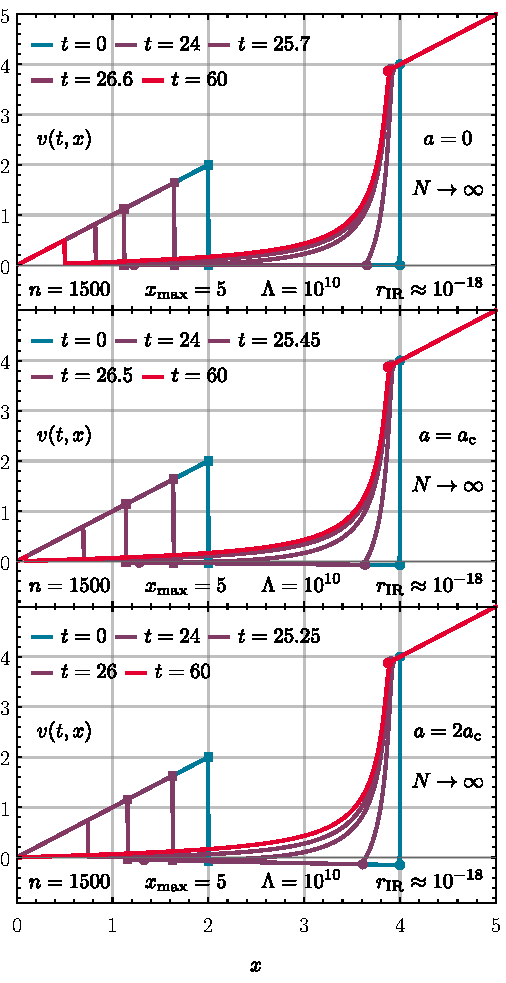
\includegraphics[width=\subcaptionFigureWidth-0.262cm]{0d/figures/largeN_flows.pdf}% figure (a)
		\captionsetup{font=footnotesize,width=\subcaptionFigureWidth-0.262cm}%
		\caption{\frg{} flow of the derivative of the rescaled effective potential $v ( t, x )$}% caption (a)
		\label{fig:frg_largeN}% label (a)
	}
	{\hspace{\subcaptionFigureSpacing}}% spacing
	{% figB
		\raisebox{-0.102cm}{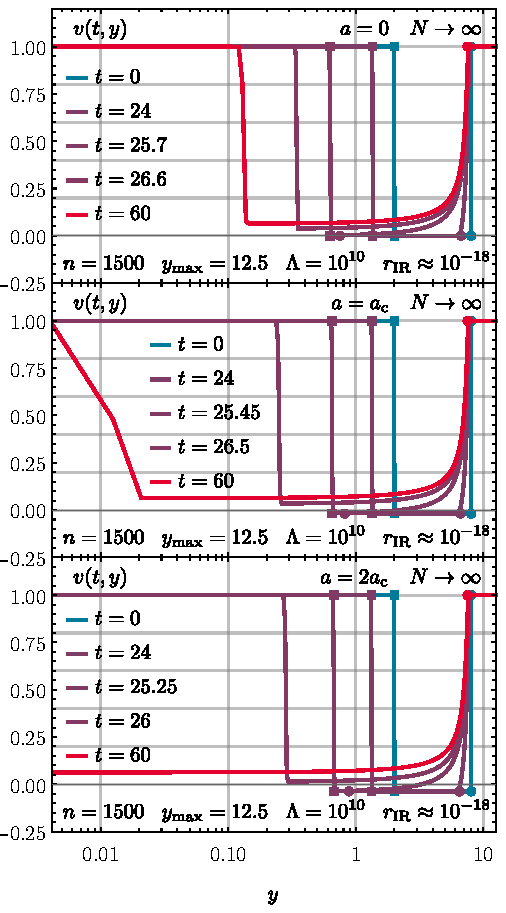
\includegraphics[width=\subcaptionFigureWidth+0.262cm]{0d/figures/largeN_KNPO1flows.pdf}}% figure (b)
		\captionsetup{font=footnotesize,width=\subcaptionFigureWidth+0.262cm}%
		\caption{%
			\frg{} flow of the derivative of the rescaled effective potential $v ( t, y )$.
			We choose a logarithmic scale for the $y$-axis for better visibility around $y = 0$ which is particularly useful for the visualization of the freezing shocks in the \ir{} for $a = 0$ and $a = a_\mathrm{c}$.%
		}% caption (b)
		\label{fig:frg_largeN_KNPO1_flows}% label (b)
	}
	{%
		\frg{} flows for the zero-dimensional $O(N)$ model in $x$ on the left \subref{fig:frg_largeN} and in the $\tfrac{1}{N}$-rescaled invariant $y \equiv \tfrac{1}{2} \, x^2$ on the right \subref{fig:frg_largeN_KNPO1_flows} in the limit $N \rightarrow \infty$ for the \ic{}~\eqref{eq:RP_vofx} with ${a = 0}$, ${a = a_\mathrm{c}}$, and ${a = 2 a_\mathrm{c}}$ in the upper, middle, and lower panel respectively.
		{Blue} curves represent the \uv{} initial conditions at $t=0$, {red} curves correspond to the \ir{} potentials at $t = 60$ and the {violet} curves are at intermediate, selected \rgtimes{} $t$ chosen around the respective collision of the shock $\xi_\mathrm{s} ( t ) $ with the left tip of the rarefaction fan $\xi_\mathrm{r}^{-}(t)$.
		The squares mark the shock $( \xi_\mathrm{s} ( t ), v ( t, \xi_\mathrm{s} ( t )^\pm ) )$, while the disks mark the tips of the rarefaction fan $( \xi_\mathrm{r}^\pm ( t ), v ( t, \xi_\mathrm{r}^\pm ( t ) ) )$.
		The left tip of the rarefaction fan and the shock are only marked up to the \rgtime{} when they meet since the underlying analysis based on the method of characteristics and Rankine-Hugoniot condition breaks down after their collision.
		\fromFigs{5 and 10}{zerod3}%
	}% caption
	{fig:frg_largeN_flows}% label
Next, we apply the \kt{} scheme~\cite{KTO2-0} from numerical fluid dynamics to the problem posed by the \pde{} \eqref{eq:frg_flow_Ninf_x} with initial condition \eqref{eq:RP_vofx}.
The corresponding (numerical) parameters are either incorporated in the figures or their corresponding captions.
Additionally, we discuss the choice of some of our (numeric) parameters and some aspects of the implementation in \LargeNnumApp{}.

We obtain the following numeric results for the \frg{} flows of $v ( t, x )$: In \cref{fig:frg_largeN} we plot the \frg{} flow of $v ( t, x )$ from the \uv{} initial condition \eqref{eq:RP_vofx} (see \cref{fig:Vofx}) at $t = 0$ to the \ir{} at $t \rightarrow \infty$. 
Of course, for practical (numerical) calculations one has to stop the integration at some finite $t$ in the \ir{}.
Here we chose $t = 60$, which corresponds to an \ir{} cutoff $r_\mathrm{IR} \approx 10^{-18}$, which is 18 orders of magnitude below model scales (which are considered to be of order one in $\tfrac{1}{N}$-rescaled quantities).
Our \uv{} scale $\Lambda$ was chosen to be ten orders of magnitude above model scales to guarantee \rgcy{}~\cite{Braun:2018svj,Koenigstein:2021syz} to a sufficient level. 
In total, we are integrating over 28 orders of magnitude in the regulator scale and corresponding tests for \uv{}-scale-independence are presented in \LargeNnumApp{}.

\Cref{fig:frg_largeN} shows \frg{} flows for $v ( t, x )$ for different values of $a$.
In the upper panel $a = 0$ and therefore clearly below $a_\mathrm{c}$, such that this \frg{} flow corresponds to the situation, where the $\tfrac{1}{N}$-expansion is applicable.
The middle panel shows the \frg{} flow exactly at the threshold $a = a_\mathrm{c}$, where the exponent \eqref{eq:fofy} has two degenerate minima \eqref{eq:saddle_minima}, with one being a non-analytic point, preventing a saddle-point expansion.
The bottom panel in \cref{fig:frg_largeN_flows} corresponds to a situation, where $a > a_\mathrm{c}$ and the saddle-point expansion again fails as it is not applicable to this initial condition.

As already mentioned at the end of the previous subsubsection, we find that the different situations within the saddle-point expansion are realized by freezing or colliding and annihilating shock waves, caused by the interplay with the rarefaction fan.
This is clearly seen in \cref{fig:frg_largeN}, where the position $\xi_\mathrm{s} ( t )$ of the shock wave is marked with squares and the positions $\xi_\mathrm{r}^- ( t )$ and $\xi_\mathrm{r}^+ ( t )$ of the tips of the rarefaction fan are marked with disks \dash{} up to the \rgtime{}, where they meet and interact rendering the analytic expressions invalid.

Explicitly, we find that for $a = 0$ (upper panel \cref{fig:frg_largeN}) the opposing shock waves ultimately freeze at ${| x | = |\xi_\mathrm{s} ( t = 60 )| \approx 0.496}$.
We obtained this value using computations at different numerical spatial resolutions $\Delta x$ by varying the number of volume cells $n$ while keeping the computational extent fixed to $x\in[0,5]$.
The explicit value of $| x | \approx 0.496$ has been extracted from the fit
	\begin{align}
		|\xi_\mathrm{s} ( t \rightarrow \infty )| \approx |\xi_\mathrm{s} ( t = 60 )| =0.496 + 0.788\, \Delta x^{0.869}\, .\label{eq:xis_0ac_fit}
	\end{align}
obtained from 41 data points with $n$ varying between $64$ and $2048$.
The non-vanishing value of ${|\xi_\mathrm{s} ( t \rightarrow \infty )|\approx 0.496}$  has the effect that the $x$-derivatives of $v ( t, x )$ at ${x = 0}$ never change during the \frg{} flow and ${\partial_x v ( t, x ) \big|_{x = 0} = 1}$ for all times $t$, while all higher $x$-derivatives vanish.
Yet, these derivatives are in direct correspondence to the \ipi{} correlation functions $\Gamma^{(n)}$, which are extracted from $v ( t, x )$ in the \ir{} at the physical point ${x = 0}$ by differentiation \wrt{}\ $x$,
	\begin{align}
		N^{\frac{n - 1}{2}} \, \Gamma^{(n + 1)} = \partial_x^n v ( t,  x ) \big|_{t \rightarrow \infty, x = 0} \, .	\label{eq:1pi_ir}
	\end{align}
Hence, although having highly non-linear dynamics involving the interaction shocks and rarefaction waves for ${|x| \smallergtrsim 0.496}$, the function $v ( t, x )$ never changed its shape for ${- 0.496 \smallerlesssim x \smallerlesssim 0.496}$ and always resembles a massive free \qft{} in this part of field space.
Metaphorically speaking and to stay in the fluid-dynamic picture: It is as if the physical point $x = 0$ in field space is ``sitting in the eye of a cyclone''.

Increasing $a$ towards the critical threshold $a_\mathrm{c}$ one observes that the shock waves freeze closer and closer to $x = 0$. Considering the metaphor of the previous paragraph, as $a$ approaches $a_\mathrm{c}$ from below the radius of the eye of the cyclone vanishes.
At $a = a_\mathrm{c}$ (middle panel \cref{fig:frg_largeN}) one still observes a freezing of the shock wave in the \ir{} at $|x| \approx 0.095$, which however is an artifact of the finite spatial resolution $\Delta x$ of the numerical scheme.
This effect can be removed by successively decreasing the \fv{} computational cells $\Delta x$. We find that for $a = a_\mathrm{c}$ the shock freezes at $x = 0$, because the shock position in the \ir{} scales as follows with $\Delta x$ for this situation,
	\begin{align}
		|\xi_\mathrm{s} ( t \rightarrow \infty )| \approx |\xi_\mathrm{s} ( t = 60 )| = 0.983\, \Delta x^{0.413}\, ,\label{eq:xis_1ac_fit}
	\end{align}
again obtained from a fit to 41 data points with the number of volume cells $n$ varying between $64$ and $2048$ while keeping $x_\mathrm{max}$ fixed.

However, as soon as $a > a_\mathrm{c}$ (middle panel \cref{fig:frg_largeN}) the interplay of the rarefaction waves and the shock waves no longer hinders the shock waves to collide and annihilate at $x = 0$. In turn, this has two direct consequences: Firstly, in the hydrodynamic language, the additional interaction of two discontinuities (the annihilation of the shock waves) again unavoidably leads to a loss of information and an abstract production of entropy on the level of the \pde{}.
This is discussed in more detail in the \customref{paragraph:infiniteNflowsY}{next paragraph}.
Secondly, in the quantum field theoretical picture the annihilation of the shock waves caused a change in the slope of $v ( t, x )$ at the physical point $x = 0$.
This directly affects the \ipi{} correlation functions, which are again extracted in the \ir{} via \cref{eq:1pi_ir}. Indeed, we find that our numeric calculations reproduce the exact results~\eqref{eq:two-point_exact} and \eqref{eq:n-point_exact}.

In summary and again metaphorically speaking, the slight change in the slope $a$ of the initial condition \eqref{eq:RP_vofx} at $t=0$ on the interval $x \in [ 2, 4 ]$ causes a tremendous change of the non-linear dynamics of the fluid $v ( t, x )$, also at other positions in field space and later \rgtimes{}, which can be seen as a ``butterfly effect'' in a \qft{}.
The small deviations in the initial condition in the \uv{} \dash{} in the metaphor the minor perturbations caused by a distant butterfly flapping its wings  \dash{} have tremendous impact on the solution in the \ir{} at the physical point \dash{} whether or not the formed cyclone has an eye or not. This further supports the notion of a first-order phase transition at $a_\mathrm{c}$ and the corresponding mechanism discussed in \ccite{Grossi:2019urj}.\bigskip
\subcaptionFigure%
	[!t]% Placement
	{0d/figures/largeN_0_flow3D.pdf}% Figure (a)
	[\caption{\frg{} flow of $v(t,x)$ for $a=0$ as 3D-plot corresponding to the flow displayed in the upper panel of \cref{fig:frg_largeN_flows}}]% Caption (a)
	{fig:largeN_0_flow3D}% label (a)
	{0d/figures/largeN_2_flow3D.pdf}% Figure (b)
	[\caption{\frg{} flow of $v ( t, x )$ for $a = 2 a_\mathrm{c}$ as 3D-plot corresponding to the flow displayed in the lower panel of \cref{fig:frg_largeN_flows}}]% Caption (b)
	{fig:largeN_2_flow3D}% label (b)
	{%
		\frg{} flows of $v ( t, x )$ for $a=0$ on the left \subref{fig:largeN_0_flow3D} and $a = 2 a_\mathrm{c}$ on the right \subref{fig:largeN_2_flow3D}.
		The left and right tips $( \xi_\mathrm{r}^\mp ( t ), t, v( t, \xi_\mathrm{r}^\mp ( t ) ) )$ of the rarefaction fan are plotted as {yellow} lines while the the shock $( \xi_\mathrm{s} ( t ), t, v ( t, \xi_\mathrm{s} ( t ))^\pm )$ is marked with {green} lines. The left tip of the rarefaction fan and the shock are only marked up to $( t, x ) \approx ( 25.718, 1.115 )$ and $( t, x ) \approx ( 25.270, 1.146 )$ in \subref{fig:largeN_0_flow3D} and \subref{fig:largeN_2_flow3D} respectively, where they meet and the analysis based on the method of characteristics and Rankine-Hugoniot condition breaks down.
		\fromFigs{6 and 7}{zerod3}%
	}% Caption
	{fig:largeN_flow3D}% Label
For a better/alternative visualization of this dynamics, we present two supplemental 3D-plots for the \frg{} flows of the upper and bottom panel of \cref{fig:frg_largeN}.
The curves from \cref{fig:frg_largeN} are slices of constant intermediate times of the 3D-plots in \cref{fig:largeN_flow3D}. 
The color coding of all figures is identical.
The attentive reader might recognize \cref{fig:largeN_0_flow3D} (without its axes) as the cover picture of this thesis.

In addition to this rather qualitative discussion, we also provide explicit numerical errors, which can be used to judge to quality of the \kt{} scheme~\cite{KTO2-0} and our implementation in the context of \frg{} flows. 
In \cref{tab:KT1500errors} we list the relative errors of the \ipi{} two-point function $\Gamma^{(2)}$ extracted from the numerical \frg{} flows of $v ( t, x )$ using \cref{eq:derivative_1_central_error_2} and the exact results \eqref{eq:two-point_exact} with \eqref{eq:n-point_exact} as reference values.

We close our discussion on the analysis of the infinite-$N$ \frg{} flows by noting that, in contrast to the $\tfrac{1}{N}$-saddle point expansion or perturbative methods, the \frg{} in its fluid-dynamic framework is applicable and also produces reliable results in a highly non-perturbative regime.
Furthermore, the \frg{}-fluid-dynamic framework, naturally copes with different kinds of non-analyticities, while all kind of ``expansion-type'' methods tend to collapse in the vicinity of relevant non-analytical physics that is only correctly described by fully fledged non-perturbative setups, \cf{} \cref{subsubsec:sc2,subsubsec:sc3}.

\paragraph{Numerical results at infinite \texorpdfstring{$N$}{N} in \texorpdfstring{$y$}{y}}\phantomsection\label{paragraph:infiniteNflowsY}\mbox{}\\%
In \cref{fig:frg_largeN_KNPO1_flows} we present numerical results for the \frg{} flow in the rescaled invariant $y$ using the flow equation \eqref{eq:frg_flow_Ninf_y} with the piecewise constant initial condition of \cref{eq:RP_vofy} obtained with the \knp{} $\order ( \Delta y^1 )$ scheme discussed in the \customref{paragraph:knpLargeN}{previous paragraph}.
The flow equation \eqref{eq:frg_flow_Ninf_y} with the piecewise constant initial condition of \cref{eq:RP_vofy} constitutes two Riemann problems as outlined in \cref{paragraph:RP}.
The \frg{} flows in $y$ displayed in \cref{fig:frg_largeN_KNPO1_flows} are equivalent to the ones in $x$ presented in \cref{fig:frg_largeN} hence we will not repeat the preceding qualitative discussion.
In the following we will instead focus on certain aspects and problems inherent to the formulation and solution in the rescaled invariant $y$.\bigskip
	
For small \rgtimes{} $t \smallerlesssim 25$ the \frg{} flows present as typical Riemann problems with a moving shock wave and a rarefaction fan, \cf{} our discussion of Euler equations in \cref{subsec:hydroEuler}. 
In \cref{fig:frg_largeN_KNPO1_flows} the evolution for $t \smallerlesssim 25$ is for all $a$ under consideration similar to the dynamics studied in Fig.~2~(a) of \ccite{Grossi:2019urj}, which originally motivated the chosen initial condition in this work.
Beyond $t \approx 25$ the shock wave and the left tip of the rarefaction fan start interacting leading to a freeze-out of the shock wave for $a = 0$ with ${v ( t = 0, y = 0 ) = 1 = \partial_x v ( t = 0, x ) \big|_{x = 0}}$.

For $a=2a_\mathrm{c}$ the shock moves out of the computational domain at $y=0$ and we recover ${v(t=0,y=0)=\frac{1}{16}=\partial_x v(t=0,x)\big|_{x = 0}}$. So far in complete agreement with the corresponding results in $x$ of \cref{paragraph:infiniteNflows}.

For $a=a_\mathrm{c}$ we observe the remnant of the shock wave in the computational interval but the shock is strongly deformed by numerical(!) diffusion/the finite resolution of the computation.
The situation at $a=a_\mathrm{c}$ can be understood quite easily.
The presented numerical computations use ${n=1500}$ volume cells equidistantly distributed in the interval ${y \in [ 0, 12.5 ]}$ resulting in ${\Delta y = \frac{1}{120} \simeq 8.33 \cdot 10^{-3}}$. 
Consequently the first two volume cells are centered at ${y_0 = \frac{1}{240} \simeq 4.17 \cdot 10^{-3}}$ and ${y_1 = \frac{1}{80} = 1.25 \cdot 10^{-2}}$.
Those two volume cells are clearly visible in the middle panel of \cref{fig:frg_largeN_KNPO1_flows} and contain the frozen shock for ${a = a_\mathrm{c}}$.
From our computation in $x$ we found with the fit \eqref{eq:xis_1ac_fit} that the shock for $a = a_\mathrm{c}$ approaches $x = 0$ with $0.983 \, \Delta x^{0.413}$.
For ${n = 1500}$ volume cell this amounts to a numerical shock position of ${| x | \approx 0.095}$ and consequently ${y \approx 4.513 \cdot 10^{-3}}$, which is for a computation in $y$ with ${n = 1500}$ retaining ${x_\mathrm{max} = 5 \Leftrightarrow y_\mathrm{max} = 12.5}$ approximately at the center of the first volume cell.
Having no volume cell to the right of the shock makes it numerically impossible to resolve ${v(t=0,y=0)=1=\partial_x v(t=0,x)\big|_{x = 0}}$ accurately.
Using the fit \eqref{eq:xis_1ac_fit} we can extrapolate that having the shock centered in the second or third cell would already require an extensive amount of volume cells namely ${n=3.7\cdot 10^5}$ or ${n=6.4\cdot 10^6}$ respectively while maintaining ${y_\mathrm{max}=12.5}$.
Computations with $10^5$ and more volume cells overtax our current implementation and computational capacities, see \LargeNnumApp{} for details.
Resolving dynamics at small $x$ with an equidistant grid of volume cells in $y = \tfrac{1}{2} \, x^2$ is in general difficult because equidistant cells in $y$ have a poor resolution around $x = \sqrt{2 y} = 0$.
A drastic example is the freezing shock for $a = a_\mathrm{c}$ at $x = 0$, where the scaling $\propto \Delta x^{0.413}$ is already challenging.
A situation with a scaling $\propto\Delta x^{p}$ with $p\geq\frac{1}{2}$ is also conceivable. Such a scenario would be impossible to resolve with an equidistant grid in the rescaled invariant $y = \frac{1}{2} \, x^2$.
To improve or in some cases even facilitate computations at all around $x=0$ in the rescaled invariant $y$ a non-uniform mesh in $y$ seems necessary.
The generalization of the \kt{} and \knp{} scheme to non-uniform grids is straightforward in one spatial dimension, see, \eg{}, \ccite{Kurganov2020}, but will not be discussed in this work. 

\paragraph{Entropy and irreversibility at infinite \texorpdfstring{$N$}{N}}\phantomsection\label{paragraph:infiniteNflowsEntropy}\mbox{}\\%
\fullWidthTwoColumnFigureTable%
	[!t] % Placement
	{0d/figures/TVD_Cfkt.pdf} % Figure
	{fig:frg_largeN_TVD} % Figure label
	{%
		The \frg{} flow of the $\mathcal{C}$-function, see \cref{eq:TVDentropy}, for the zero-dimensional $O(N)$~model in the limit ${N \rightarrow \infty}$ for the Riemann problem of \cref{eq:RP_vofy} with $a = 0$, $a = a_\mathrm{c}$, and $a = 2 a_\mathrm{c}$ obtained with the \knpScheme{} of $\order ( \Delta y^1 )$.
		We observe plateaus in the \uv{} and \ir{}.
		The \ir{} plateaus end for the individual values of $a = 0$, $a = a_\mathrm{c}$, and $a = 2 a_\mathrm{c}$ at the \rgtimes{} when the shock wave and rarefaction fan intersect namely at $t \approx 25.718$, $25.469$, and $25.270$ respectively. The second jump in the curves for $a \geq a_\mathrm{c}$ is due to the collision of the shock waves at $x = 0$.
		\fromFig{11}{zerod3}%
	} % Figure caption
	{%
		\renewcommand{\arraystretch}{1.15}
		\small
		\begin{tabular}{l | c c c}
			\toprule
			$N$			&	$a = 0$		&	$a = a_\mathrm{c}$	&	$a = 2\, a_\mathrm{c}$\\
			\midrule
				$\infty$	&	$8.0 \cdot 10^{-15}$	&	$1.2 \cdot 10^{-14}$	&	$3.3 \cdot 10^{-3}$\\
				$2$		&	$6.4 \cdot 10^{-5\phantom{0}}$	&	$5.5 \cdot 10^{-5}$	&	$4.5 \cdot 10^{-5}$	\\
				$32$	&	$4.2 \cdot 10^{-3\phantom{0}}$	&	$6.4 \cdot 10^{-4}$	&	$8.5 \cdot 10^{-3}$\\
			\bottomrule
		\end{tabular}
	} % Table content
	{tab:KT1500errors}% Table label
	{%
		Relative numerical errors for the \ipi{} two-point function $\Gamma^{(2)}$, see \cref{eq:derivative_1_central_error_2}, for the results plotted in \cref{fig:frg_largeN,fig:frg_N2_flows,fig:frg_N32_flows},
		with corresponding exact reference values from the last row of \cref{tab:Gamma2N}.
		The scaling of these errors with the number of volume cells can be found in Tabs. V, VIII, and IX of \ccite{zerod3} for $N\rightarrow\infty$, $N=2$, and $N=32$ for $a=2\,a_\mathrm{c}$.
		\fromTabs{II and III}{zerod3}%
	} % Table caption
We now turn to the discussion of the (numerical) entropy associated with the purely advective \frg{} flows in the rescaled invariant $y$ at infinite $N$.
In \cref{subsec:0dO1Entropy} we discussed the concept of (numerical) entropy of \frg{} flows and its relation to the inherent irreversibility of \grg{} flows in detail.
We further argued for a connection between the (numerical) entropy of \frg{} flows and Zamolodchikov's~\cite{Zamolodchikov:1986gt} or more recent~\cite{Codello:2013iqa,Codello:2015ana} formulations of the $\mathcal{C}-$function.

In \cref{subsec:0dO1Entropy} we focused on the limiting case $N=1$ of the purely diffusive zero-dimensional $O(1)$~model.
The focus of this paragraph is the opposite limit of $N\rightarrow\infty$ yielding purely advective flow equations.
While a (numerical) entropy production is almost intuitively understood for diffusive problems the present situation might seem less obvious for a non-expert reader. 
In our introduction of non-linear advection equations in \cref{paragraph:BBE} we discussed, that the appearance and/or interaction of discontinuities like shocks and rarefaction waves can be linked to an increase in numerical entropy. 
Which in turn signals the irreversibility of the underlying flow.
Defining or constructing an explicit numerical entropy functional for general non-linear conservation laws is a difficult task especially when source terms are involved, \cf{} \ccite{Monthe:2001,Beneito2008,Chen2011May,Bessemoulin:2012} and references therein. 

When considering the flow equations \eqref{eq:frg_flow_x} and \eqref{eq:frg_flow_y} in $x$ or $y$ respectively, we note that the formulation in $x$ ($y$) involves a position-dependent advection term (diffusion term).
When executing the $x$-derivative in \cref{eq:frg_flow_x} we can differentiate between three contributions in the resulting flow equation in primitive form: a parabolic diffusion term $\propto \partial_x^2 v(t,x)$ with a non-linear diffusion coefficient, a hyperbolic advection term $\propto \partial_x v(t,x)$ with a non-linear, position-dependent advection velocity $\partial_v F$ and a non-linear, position-dependent internal source term $\propto v(t,x)$ stemming from the product rule.
As a consequence of the latter term the \rhs{} of the flow \cref{eq:frg_flow_x} and hence $\partial_t v(t,x)$ is non-vanishing for $v(t,x)$ constant in $x$.
Similarly the flow \cref{eq:frg_flow_y} in $y$ contains such a non-linear, position-dependent internal source term $\propto v(t,y)$ arising from the derivative of the explicitly $y$-dependent second term in \cref{eq:frg_flow_y}. 
Those internal source terms, explicit $x$- or $y$-dependencies before executing the derivatives, in the flow equations in primitive form make the construction of explicit numerical entropy functionals at finite $N > 1$ challenging.

In \cref{subsec:0dO1Entropy} we discussed (numerical) entropy functions at length for the purely diffusive system at $N=1$.
The \tv{} had been identified as one suitable entropy functional.

Incidentally in the opposite limit $N\rightarrow\infty$ but using the flow \cref{eq:frg_flow_Ninf_y} in the rescaled invariant $y$ the \tv{}/arc-length is again a viable entropy functional.
This goes back to general properties of (weak) solutions of purely hyperbolic non-linear advection equations \dash{} like our $N\rightarrow\infty$ flow \cref{eq:frg_flow_Ninf_y}.
Among other general qualitative statements about monotonicity and convexity (weak) solutions of hyperbolic non-linear advection equations like \cref{eq:frg_flow_Ninf_y} have a decreasing arc length \dash{} they are total variation non-increasing (TVNI) as discussed in \cref{subsec:hydroKT}.
Since solutions of the underlying flow \cref{eq:frg_flow_Ninf_y} are TVNI ($\partial_t \mathrm{TV}[v(t,y)]\leq 0$) the entropy functional $\mathcal{C}$ is non-decreasing ($\partial_t\mathcal{C}\geq 0$).

Solutions of the flow \cref{eq:frg_flow_x} in $x$ at $N>1$ are in general not \tvni{}.
A fact we tested in numerical experiments with several initial conditions at various $N>1$~\cite{Koenigstein:2021syz,Koenigstein:2021rxj,Steil:2023zeroDlargeN,Steil:2023zeroDN1}.
The loss of the \tvni{} property is directly linked to the explicit position-dependencies in the flow equation manifesting as source terms when executing the $x$-derivatives of the \rhs{} of \cref{eq:frg_flow_x}.
Formal results supporting this can be found in \ccite{Redheffer1974Mar}: non-linear parabolic differential equations of the type $0=\partial_t v-f(t,z,v,\partial_z v,\partial_{z}^2 v)$ have \tvni{} solutions if (among some other restrictions) the flux $f$ vanishes, \ie{}, $0=f(t,z,v,0,0)$ on constant solutions $0=\partial_z v=\partial_{z}^2 v$.
The latter is not the case for flow equations in $x$ at $N>1$ and in $y$ for finite $N$ as discussed earlier in this subsection.
It is intuitively obvious that source terms can increase the arc length of a (weak) solution and implications in the context of \tvni{} schemes are discussed in, \eg{}, \ccite{Monthe:2001,Beneito2008,Chen2011May,Bessemoulin:2012}.

For $N \rightarrow \infty$ solutions in $x$ are still not \tvni{} but a reformulation in $y$ eliminates the explicit position-dependence in the advection flux and the resulting source term.
The solutions of the flow \cref{eq:frg_flow_Ninf_y} in $y$ are \tvni{}.
A fact we tested numerically, see \cref{fig:frg_largeN_TVD}, for the Riemann problems posed by the initial condition~\eqref{eq:RP_vofy} with the flow \cref{eq:frg_flow_Ninf_y} and which is theoretically well established \cf{}~\ccite{HARTEN1983357,Lax1973}.\bigskip

We conclude this subsubsection with a qualitative discussion of the numerical entropy for the Riemann problems posed by the initial condition~\eqref{eq:RP_vofy} with the flow \cref{eq:frg_flow_Ninf_y} for different $a$.
The numerical entropies associated to the flows presented in \cref{fig:frg_largeN_KNPO1_flows} are plotted in \cref{fig:frg_largeN_TVD}.

The numerical entropy stays constant in the \uv{} up until the point where the shock wave and rarefaction fan intersect namely at $t \approx 25.718$, $25.469$, and $25.270$ for $a = 0$, $a = a_\mathrm{c}$, and $a = 2 a_\mathrm{c}$ respectively.
Since both shock and rarefaction wave are already present in the initial condition $v(t=0,y)$ their simple advection does not increase the numerical entropy of \cref{eq:TVDentropy}.
The flow in the \uv{} is therefore arguable reversible, which can be seen from the analytic solutions via the method of characteristics, but practical computations involving a finite resolution $\Delta y$ and finite precision during time evolution prevent an accurate reversion by numerically integrating up in time $t$.

Between $t \approx 25$ and $t \approx 35$ we observe an increase in numerical entropy related to the interaction of the shock and the rarefaction fan.
For $a\leq a_\mathrm{c}$ the rise in entropy is rather small related to only marginal changes in arc length/\tv{} during the flow, see upper and middle panel of \cref{fig:frg_largeN_KNPO1_flows}.
For $a>a_\mathrm{c}$ namely $a=2a_\mathrm{c}$ we observe a steep rise in entropy at $t\approx 27.275$, which is the \rgtime{} at which the shock leaves the computational domain for $a=2a_\mathrm{c}$. Without the shock the arc length/\tv{} decreases dramatically leading to the observed rise in numerical entropy.

In the \ir{} for $t \smallergtrsim 35$ we again observe a plateau in the numerical entropy, related to the fact, that $k(t)$ for $t \smallergtrsim 35$ is sufficiently below the internal model scales of the problem under consideration meaning that all relevant fluctuations are already included.
The plateaus in the numerical entropy in the \uv{} and \ir{} are indicators of \rgcy{} and sufficiently small numerical \ir{} cutoffs respectively.

\FloatBarrier
\subsubsection{FRG flows at finite \texorpdfstring{$N$}{N} -- diffusion as a game changer}\label{subsubsec:FRGlargeNfin}
\begin{disclaimer}
	This subsubsection follows Sec.~IV.F of \nbccite{Steil:2021cbu}.
\end{disclaimer}
\subcaptionFigure%
	[!t]% Placement
	{0d/figures/N32_flows.pdf}% Figure (a)
	[\caption{\frg{} flow with $N = 32$ for the \ic{}~\eqref{eq:RP_vofx} with $a = 0$, $a = a_\mathrm{c}$, and $a = 2 a_\mathrm{c}$ in the upper, middle, and lower panel respectively.}]% Caption (a)
	{fig:frg_N32_flows}% label (a)
	{0d/figures/N2_flows.pdf}% Figure (b)
	[\caption{\frg{} flow with $N = 2$ for the \ic{}~\eqref{eq:RP_vofx} with $a = 0$, $a = a_\mathrm{c}$, and $a = 2 a_\mathrm{c}$ in the upper, middle, and lower panel respectively.}]% Caption (b)
	{fig:frg_N2_flows}% label (b)
	{%
		The \frg{} flow of the derivative of the rescaled effective potential $v ( t, x )$ for the zero-dimensional $O(N)$~model for $N=32$ on the left \subref{fig:frg_N32_flows} and $N=2$ on the right \subref{fig:frg_N2_flows}.
		{Blue} curves represent the \uv{} initial conditions at $t = 0$, {red} curves correspond to the \ir{} potentials at $t = 60$ and the {violet} curves are at intermediate, selected \rgtimes{} $t$.
		\fromFigs{8 and 9}{zerod3}%
	}% Caption
	{fig:Nfinite_flows}% Label
Next, we turn to the \frg{} flows of our initial potential \eqref{eq:RP_Vofy} at finite $N$.
To this end, we use the fluid-dynamic \frg{} flow equation \eqref{eq:frg_flow_x} including advective and diffusive contributions by the pions and the \sigmaMode{}.
As explained above, we cannot use \cref{eq:frg_flow_y} in the presence of diffusion, because the problem of diffusive influx at the $(y = 0)$-boundary, if formulated in $y$, is not settled yet to our satisfaction, \cf{} again \cref{subsec:boundary_conditions_finite_volume}.
For the following discussions at finite $N$ we hence use \cref{eq:frg_flow_x} in $x$ and the robust \kt{} scheme.
	
The main scope of this subsubsection is to demonstrate the astonishing role of the radial \sigmaMode{} in terms of highly non-linear and unconventional diffusion in \frg{} flows of scale-dependent effective potentials $V ( t, x )$ or rather their derivatives $v ( t, x ) = \partial_x V ( t, x )$.
To this end, let us again focus solely on the purely diffusive contribution of the \frg{} flow equation \eqref{eq:frg_flow_x} and rewrite it in terms of a non-linear heat equation by executing the $\sigma$-derivative on the \rhs{},
	\begin{align}
		\partial_t v ( t, x ) &= \, \dod{}{x}\! \bigg[ \ldots + \frac{1}{N} \, \frac{\tfrac{1}{2} \, \partial_t r ( t )}{r ( t ) + \partial_x v ( t, x )} \bigg] 
		= \, \ldots + \alpha [ t, \partial_x v ] \, \partial_x^2 v ( t, x ) \, , \nonumber
	\end{align}
where we again recovered the manifestly positive diffusion coefficient (note the definition \eqref{eq:exponential_regulator} of the regulator $r ( t )$ and the rescalings),
	\begin{align}
		\alpha [ t, \partial_x v ] \equiv - \frac{1}{N} \, \frac{\tfrac{1}{2} \, \partial_t r ( t )}{[ r ( t ) + \partial_x v ( t, x ) ]^2} \, ,	\label{eq:diffusion_coefficient_resc}
	\end{align}
\cf{} \cref{eq:diffusion_coefficient} for the unrescaled/original diffusion coefficient.
The identification of the sigma loop as a parabolic, diffusive contribution has severe conceptual implications.
The diffusive contribution to the flow of $v ( t, x )$ clearly introduces a dissipative process into the \frg{} flow and renders it manifestly irreversible, see again \cref{subsec:0dO1Entropy} for further details.
	
In the context of this work, however, we are mainly interested in the influence of the non-linear diffusion on the explicit shape of $v ( t, x )$ and its drastic consequences for the reliability of $\tfrac{1}{N}$-expansions and the infinite-$N$ limit.
To this end, we present our numerical solutions of \cref{eq:frg_flow_x} with initial condition \eqref{eq:RP_vofx} (see \cref{fig:Vofx}) for two choices of $N$. 
\WlogA{} we choose $N = 2$ and $N = 32$ and present respective \frg{} flows for $a = 0$, $a = a_\mathrm{c}$, and $a = 2 a_\mathrm{c}$ in \cref{fig:Nfinite_flows}.
The \cref{fig:frg_N2_flows,fig:frg_N32_flows} are structured analogously to \cref{fig:frg_largeN} (for infinite $N$).
For our numerical computations we used the same \uv{} and \ir{} cutoffs as for the infinite-$N$ case.
Nevertheless, we had to change the size of the computational interval from~${[0, 5]}$ to~${[ 0, 10 ]}$ in order to exclude boundary effects due to the diffusion.
Furthermore, it suffices to use $n = 1000$ volume cells on this interval, because it is no longer necessary to resolve the sharp shock fronts at extremely high resolution to obtain small numerical errors.
For details on these two aspects, we refer to our detailed discussion of \cref{subsec:0dONresults}.\bigskip

Qualitatively, we observe the following: Even though $N = 32$ seems to be rather large\footnote{%
Especially in the context of the large-$N_\mathrm{color}$/$N_\mathrm{flavor}$ discussions in the context of \qcd{}, \qcd{}-inspired models, or holographic methods, where $N$ is typically between $1$ and $6$.%
} the \frg{} flow of the $\tfrac{1}{N}$-rescaled $v ( t, x )$ entirely changes, if one compares corresponding panels of \cref{fig:frg_N32_flows,fig:frg_largeN} directly.
Although the underlying shock, stemming from the still rather strong advective \pionModes{}, dominates the overall shape of $v ( t, x )$ in \cref{fig:frg_N32_flows} for all three choices of $a$, the diffusive character sets in rather early during the beginning of the \frg{} flow and smears out the infinite negative slope of $v ( t, x )$ at the shock front.
Inspecting the non-linear diffusion coefficient \eqref{eq:diffusion_coefficient_resc} this is expected for all finite $N$.
Huge negative gradients $\partial_x v ( t, x )$ lower the difference $r ( t ) + \partial_x v ( t, x )$, which in turn drastically increases the diffusion coefficient leading, in combination with large $\partial_x^2 v ( t, x )$, to strong diffusion in regions where $v ( t, x )$ has large negative slopes, \eg{},\ next to the shock front.
On the other hand, if $\partial_x v ( t, x )$ has large positive slope, as is the case close to the rarefaction fan, the diffusion coefficient is drastically suppressed, even if $\partial_x^2 v ( t, x )$ is large, such that the advection still dominates close to the rarefaction wave.
For large $x \gg 5$ both, $\alpha [ t, \partial_x v ]$ and $\partial_x^2 v ( t, x )$ tend to zero (as is the case for $\tfrac{1}{x} \, v ( t, x )$ for the advection).
For all other regions in $x$ we find complicated variations of these conceptual behaviors.
	
Concerning the freezing or colliding of the shock wave, which was observed for infinite-$N$ in \cref{fig:frg_largeN_flows}, we find that remnants of the freezing shocks are still visible in Figs.~\ref{fig:frg_N32_flows} (upper and middle panel).
However, the gradient $\partial_x v ( t, x )$ no longer changes its sign at the right of the remnants of the freezing shock waves, such that overall the potential $V ( t, x )$ turns convex in the \ir{}.\bigskip
	
Turning to \cref{fig:frg_N2_flows} for the $N = 2$ scenario, where only one $\pi$- and one \sigmaMode{} are included in the calculation, we find that the overall the dynamics is very similar to the $N = 32$, but even more dominated by the diffusive contribution to the \frg{} flow.
The freezing shock waves are no longer visible in the \ir{} for $a = 0$ and $a = a_\mathrm{c}$ and the rarefaction wave is totally washed out.
The latter effect is the reason, why the computational interval had to be increased.
	
Before we turn to the overall interpretation of these findings, we remark that we also compared our numerical results for the \ipi{} two-point functions for all three choices of $a$ and $N = 2$ and $N = 32$ against exact results.
In \cref{tab:KT1500errors} we present the corresponding relative errors which are discussed further in \LargeNnumApp.\bigskip

In summary, we find that the radial \sigmaMode{} and the corresponding diffusion is a game changer in a \qft{} when switching from infinite to finite $N$. 
By directly comparing the infinite-$N$ and finite-$N$ results of the \frg{} flows, we observe that for infinite-$N$ the $\tfrac{1}{N}$-rescaled potential $V ( t, x )$ does not turn convex in the \ir{} and may still involve non-analyticities in terms of cusps.
This is in direct opposition to the zero-dimensional version of the \cmwhTheoremWithRefs{}, which states that the zero-dimensional \ir{} potential has to be convex and smooth.
On the other hand, we find that independent of the specific choice of $N$ \dash{} as long as $N$ is finite \dash{} the highly non-linear diffusion of the \sigmaMode{} restores convexity and smoothness of the \ir{} potential.
Depending on the specific choice of $N$ this may however happen at later times in the \frg{} flow, respectively at lower \rgscales{}, thus deeper in the \ir{}.
This situation is very similar to the one we encounter in our studies in the \gnym{} at finite $N$, see \cref{subsubsec:variableN} for details.
We conclude from these non-perturbative \frg{} studies, that calculations at infinite-$N$ and large-$N$, may lead to totally different results for certain aspects of a \qft{}.
This can by no means be considered a novel insight \dash{} however the \frg{} \cfd{} aspects in this context are.

	
